\vspace{0.5cm}
\subsection{Experimento 1: Experiencias con osciloscopio analógico}

\vspace{0.5cm}
\subsubsection{Aprendiendo a calibrar (compensar) la punta atenuadora}

Con este primer experimento, se pretende demostrar la importancia de la calibración de la punta de medición mediante una comparativa entre los tres tipos posibles de compensación (figura \ref{calib}).

%figura de los tres tipos de compensación

\begin{figure}[H]
    \centering
    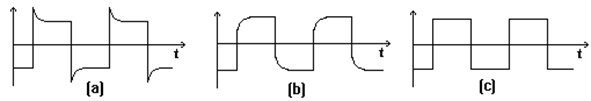
\includegraphics[width=\textwidth]{Imagenes/calib.png}
    \caption{Tipos de compensación con la punta de osciloscopio}
    \label{calib}
\end{figure}

Para comenzar, se puso el seleccionador de la punta en la opción de "X10", esto con el fin de aumentar considerablemente su resistencia de entrada al osciloscopio y disminuir su capacidad paralela de entrada, reduciendo al mínimo la influencia de la conexión del instrumento sobre el circuito a medir.

Se procedió a ajustar el capacitor de compensación en el conector de la punta hasta lograr cada una de las formas de onda. %indicas en la figura \ref{}. 

Los parámetros del osciloscopio fueron ajustados de la siguiente manera (tabla \ref{tab:cont1}):

\begin{table}[H]
    \centering
    \scalebox{1}{
    \begin{tabular}{|c|c|c|c|c|}
    \hline
         V/div (C. Y1) & t/div (B. tiempo) & Aten. Y1 & Acoplamiento & Disparo \\
    \hline
        50 $mV$ & 0.2 $ms$ & x10 & CC & CH1\\
    \hline
        \end{tabular}}
        \def\tablename{Tabla} 
        \caption{Cuadro de Controles}
        \label{tab:cont1}
\end{table}

Las señales obtenidas, se presentan a continuación (figura \ref{compen})

%foto triple de las señales del osc

\begin{figure}[H]
    \begin{center}
        \begin{subfigure}[t]{0.5\textwidth}
        \centering  
        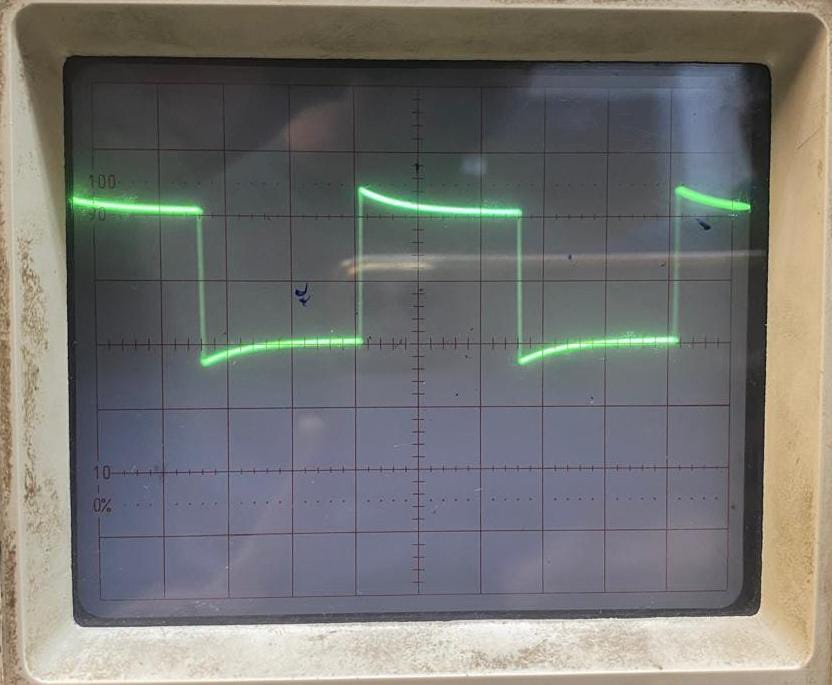
\includegraphics[width=0.75\textwidth]{Imagenes/SigA.jpeg}
        \caption{Compensación A}
        \label{fig:sigA}
    \end{subfigure}
    \hfill
    \begin{subfigure}[t]{0.49\textwidth}
        \centering
        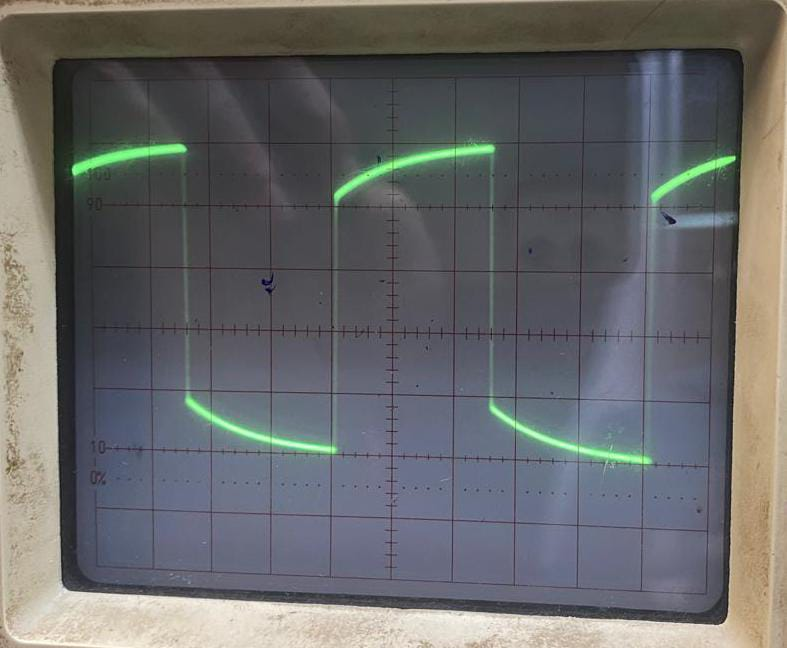
\includegraphics[width=0.77\textwidth]{Imagenes/SigB.jpeg}
        \caption{Compensación B}
        \label{fig:sigB}
    \end{subfigure}
    \begin{subfigure}[t]{0.5\textwidth}
        \centering
        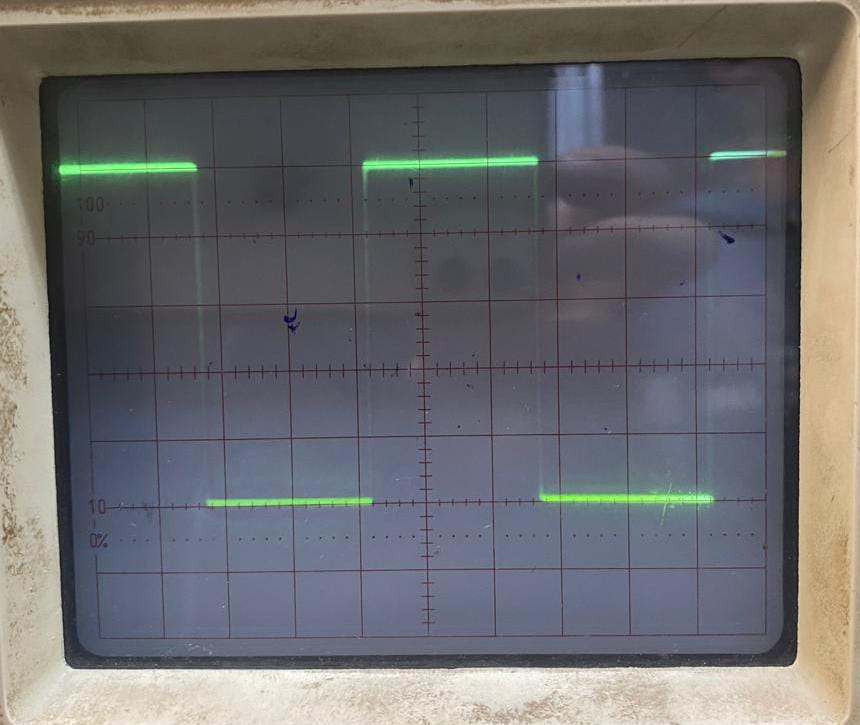
\includegraphics[width=0.75\textwidth]{Imagenes/SigC.jpeg}
        \caption{Compensación C (punta calibrada)}
        \label{fig:sigC}
    \end{subfigure}
    \caption{Señal de prueba con los tres tipos de calibración}
    \label{compen}
    \end{center}
\end{figure}

Una vez obtenida la señal de la figura \ref{fig:sigA}, se procedió a conectar un generador de funciones configurado para generar una onda sinusoidal y se realizó un barrido manual de frecuencia, desde 100 Hz hasta 1 MHz. Se tomó nota de la amplitud observada en cada instancia de frecuencia y se confeccionó una tabla con los datos. 

Debido a que había que realizar el mismo procedimiento para los tres tipos de compensación, se decidió ubicar todos los datos en una misma tabla para mayor legibilidad y para poder comparar los efectos en cada caso con mayor facilidad.

Para el barrido, se empleó una señal sinusoidal de 1 Vpp (que será visto como 100 mVpp por la punta al estar en X10), y la frecuencia fue variada según lo que se observa en la tabla. Para esta parte también se cambió la escala del osciloscopio a 20 mV/div para poder apreciar con más detalle los cambios de amplitud.

%Tabla de barrido de frecs

\begin{table}[H]
    \centering
    \scalebox{1}{
    \begin{tabular}{|c||c||c|c|c|}
    
    \hline
         \multirow{2}{*}{$f$ [Hz]} & \multirow{2}{*}{t/div [$\mu$s]} & \multicolumn{3}{c|}{Amplitud $[mVpp]$} \\
    \cline{3-5}
          &  & Comp. a) & Comp. b) & Comp. c) \\
    \hline
        100 & 2000 & 100 & 100 & 100 \\
        1k & 200 & 112 & 90 & 100 \\
        10k & 20 & 120 & 84 & 100 \\
        100k & 2 & 120 & 82 & 100 \\
        250k & 1 & 120 & 81 & 100 \\
        1M & 0.2 & 120 & 80 & 100 \\ 
    \hline
        \end{tabular}}
        \def\tablename{Tabla} 
        \caption{Barrido en frecuencia para las distintas compensaciones}
        \label{tab:BarrFrec}
\end{table}

Se puede ver, en base a los valores obtenidos, que en el único modo de compensación en el que las mediciones no variaron al cambiar la frecuencia, fue con el modo \textit{c)} (figura \ref{fig:sigC}). En los otros dos modos, la señal de entrada al osciloscopio se vio afectada por la variación de frecuencia, aumentando el valor de la señal medida en el modo \textit{a)} y disminuyéndolo en \textit{b)}.

En la hoja de enunciados se solicitaba completar una serie de frases con cada modo y estas quedan de la siguiente manera:

\begin{enumerate}
    \item El oscilograma \textbf{\textit{b)}} corresponde a “caída de respuesta en frecuencias elevadas”.
    \item El oscilograma \textit{\textbf{a)}} corresponde a “exceso de respuesta en frecuencias elevadas”.
    \item El oscilograma \textbf{\textit{c)}} corresponde a “respuesta plana”.
\end{enumerate}





\vspace{0.5cm}
\subsubsection{Acoplamiento \textit{CC/CA} de la entrada vertical (eje Y)}

En este ensayo se pretende visualizar el efecto de la capacitancia de entrada del osciloscopio cuando este se encuentra en acoplamiento de \textit{CA}.

En este modo, la entrada del eje Y del osciloscopio tiene conectado internamente, un capacitor en serie que bloquea la componente de \textit{CC} y este en ciertos casos (sobre todo a bajas frecuencias) puede provocar deformaciones en la forma de la onda. 

Para este experimento, se empleará nuevamente un generador de onda, pero esta vez se inyectara una onda cuadrada, con frecuencia de 50 Hz y amplitud de 20 $V_{pp}$ (máxima del generador). 

Inicialmente las configuraciones del osciloscopio y la punta serán las siguientes:

\begin{table}[H]
    \centering
    \scalebox{1}{
    \begin{tabular}{|c|c|c|c|}
    \hline
         V/div (C. Y1) & t/div (B. tiempo) & Aten. Y1 & Disparo \\
    \hline
        5 $V$ & 2 $ms$ & x1 & LINE\\
    \hline
        \end{tabular}}
        \def\tablename{Tabla} 
        \caption{Cuadro de Controles}
        \label{tab:cont2}
\end{table}

Se establece como fuente de disparo la opción \textit{LINE}, ya que la tensión de línea tiene una frecuencia de 50 Hz, coincidente con la señal producida por el generador. Esto debería garantizar la estabilidad de la imagen a la hora de verla en el osciloscopio.

Primeramente se selecciona la opción de acoplamiento en \textit{CC} y como era de esperarse, se muestra en pantalla una señal cuadrada sin distorsión. (figura \ref{dcx1}).

Luego se pasa a la opción de acoplamiento de \textit{CA}, la cual deforma la onda y donde antes se veían lineas horizontales (picos y valles), ahora se ven líneas con pendientes (figura \ref{acx1}).

%Imagen de las dos ondas (subfigure)

\begin{figure}[H]
    \begin{center}
        \begin{subfigure}[b]{0.5\textwidth}
        \centering  
            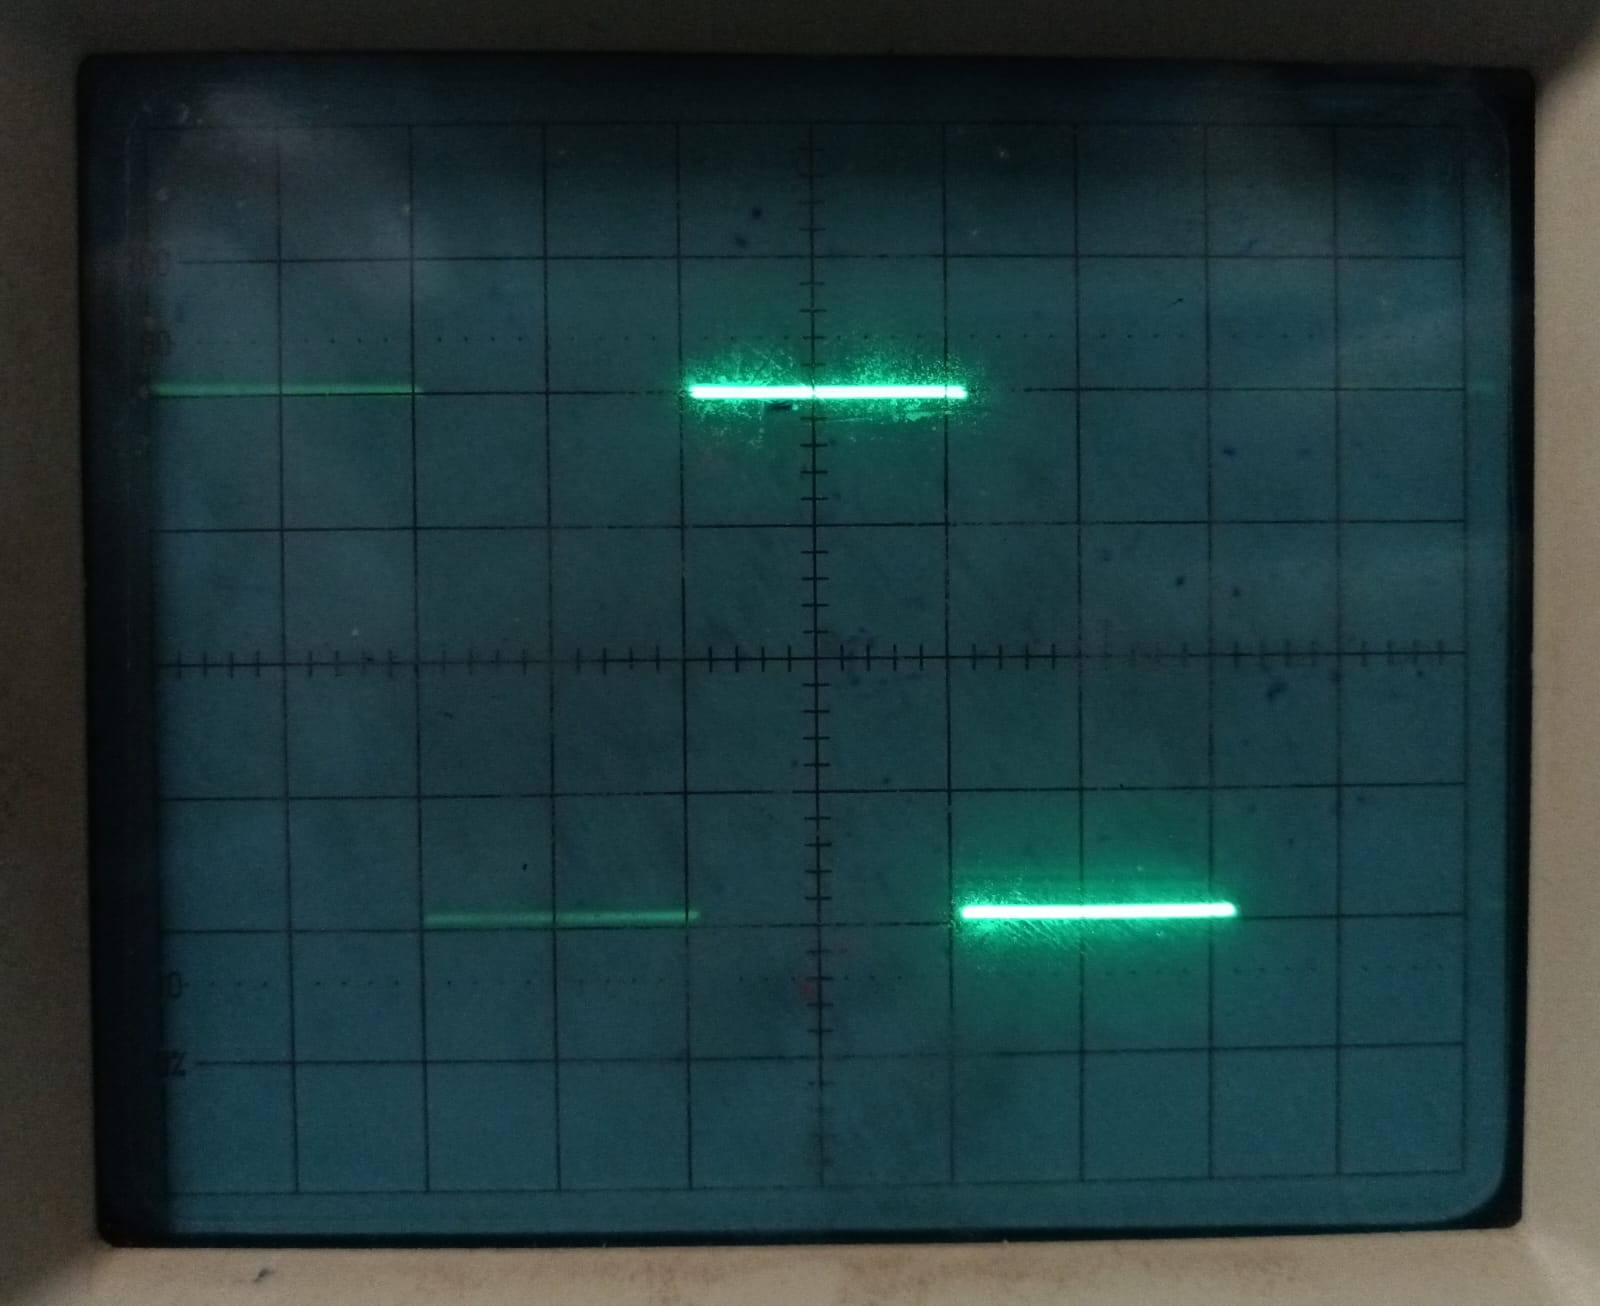
\includegraphics[width=0.75\textwidth]{Imagenes/DCx1.jpeg}
        \caption{Acoplamiento en CC}
        \label{dcx1}
    \end{subfigure}
    \hfill
    \begin{subfigure}[b]{0.49\textwidth}
        \centering
            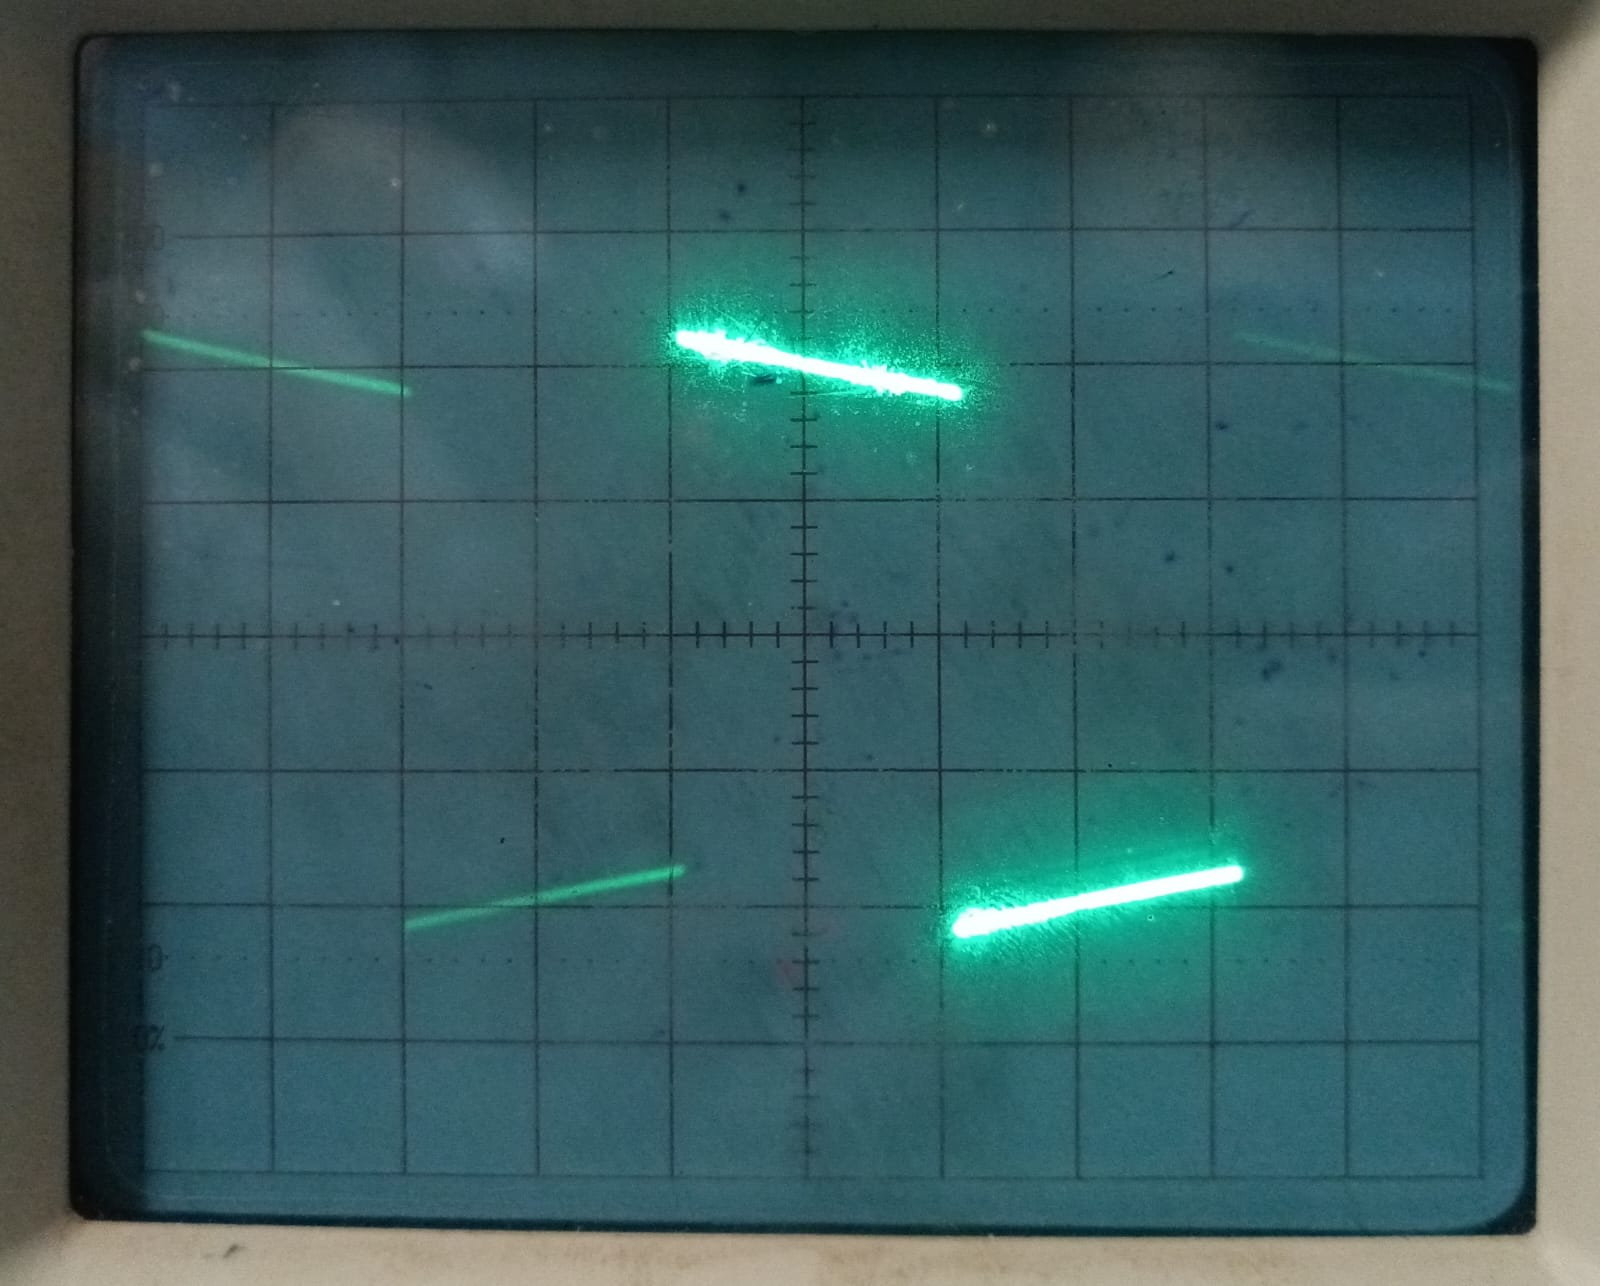
\includegraphics[width=0.77\textwidth]{Imagenes/ACx1.jpeg}
        \caption{Acoplamiento en CA}
        \label{acx1}
    \end{subfigure}
    \caption{Señal de prueba con distintos acoplamientos y punta en atenuación x1}
    \end{center}
\end{figure}

En las imágenes se ven algunos pulsos más luminosos que otros debido a que al ser una frecuencia tan baja (50 Hz), la cámara que tiene una frecuencia de muestreo de 60 Hz, sacaba las fotos tan "rápido" que la imagen no llegaba a completarse.  

Para tratar de mitigar el efecto de este capacitor de entrada, se nos propuso cambiar la atenuación de la punta a \textit{x10}, manteniendo la onda del generador. También se actualizaron las configuraciones del osciloscopio para ver correctamente la señal (tabla \ref{tab:cont2b}).

\begin{table}[H]
    \centering
    \scalebox{1}{
    \begin{tabular}{|c|c|c|c|}
    \hline
         V/div (C. Y1) & t/div (B. tiempo) & Aten. Y1 & Disparo \\
    \hline
        500 $mV$ & 2 $ms$ & x10 & LINE\\
    \hline
        \end{tabular}}
        \def\tablename{Tabla} 
        \caption{Cuadro de Controles}
        \label{tab:cont2b}
\end{table}

Nuevamente, conectamos el generador y pusimos el acople en \textit{CC} y en \textit{CA}. Los resultados se pueden ver en la figura \ref{fig:x10}.

%Imagen de las ondas con la punta en x10 (subfigure)

\begin{figure}[H]
    \label{fig:x10}
    \begin{center}
        \begin{subfigure}[b]{0.5\textwidth}
        \centering  
            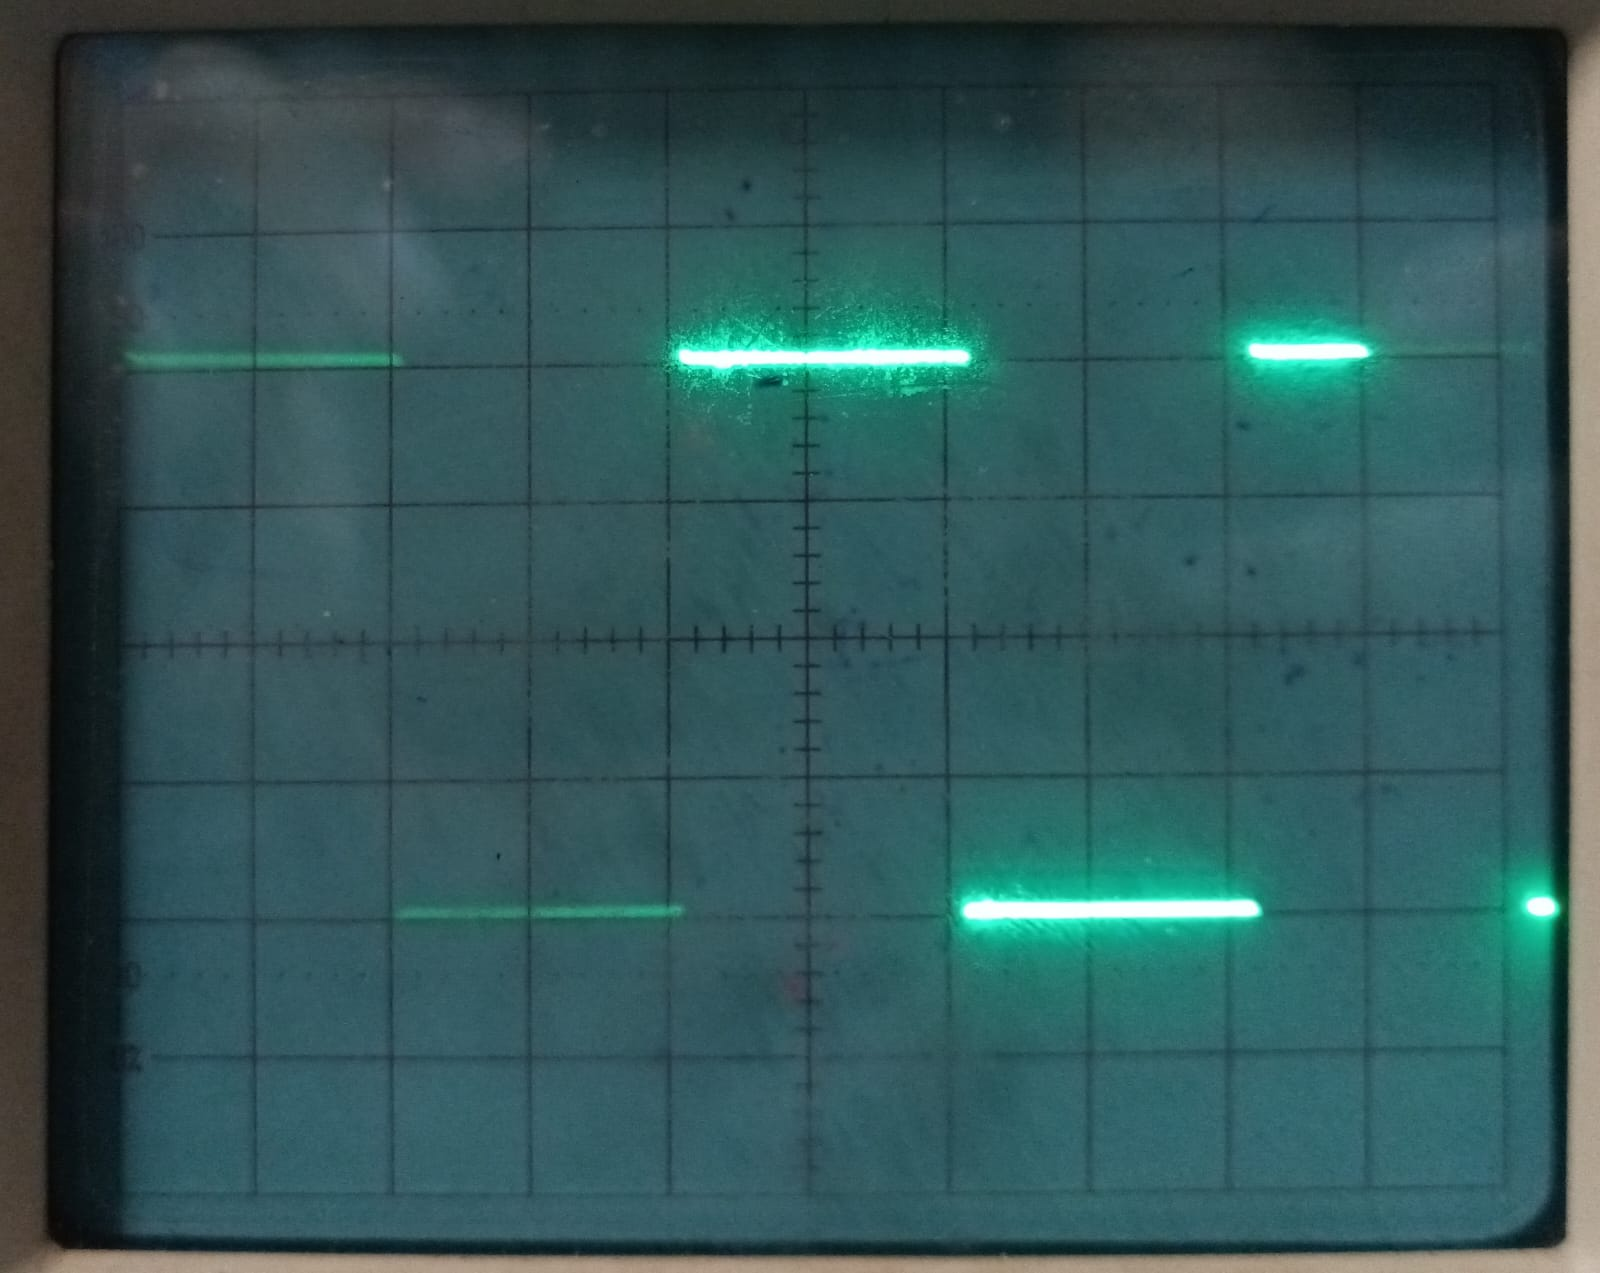
\includegraphics[width=0.75\textwidth]{Imagenes/DCx10.jpeg}
        \caption{Acoplamiento en CC}
        \label{dcx10}
    \end{subfigure}
    \hfill
    \begin{subfigure}[b]{0.49\textwidth}
        \centering
            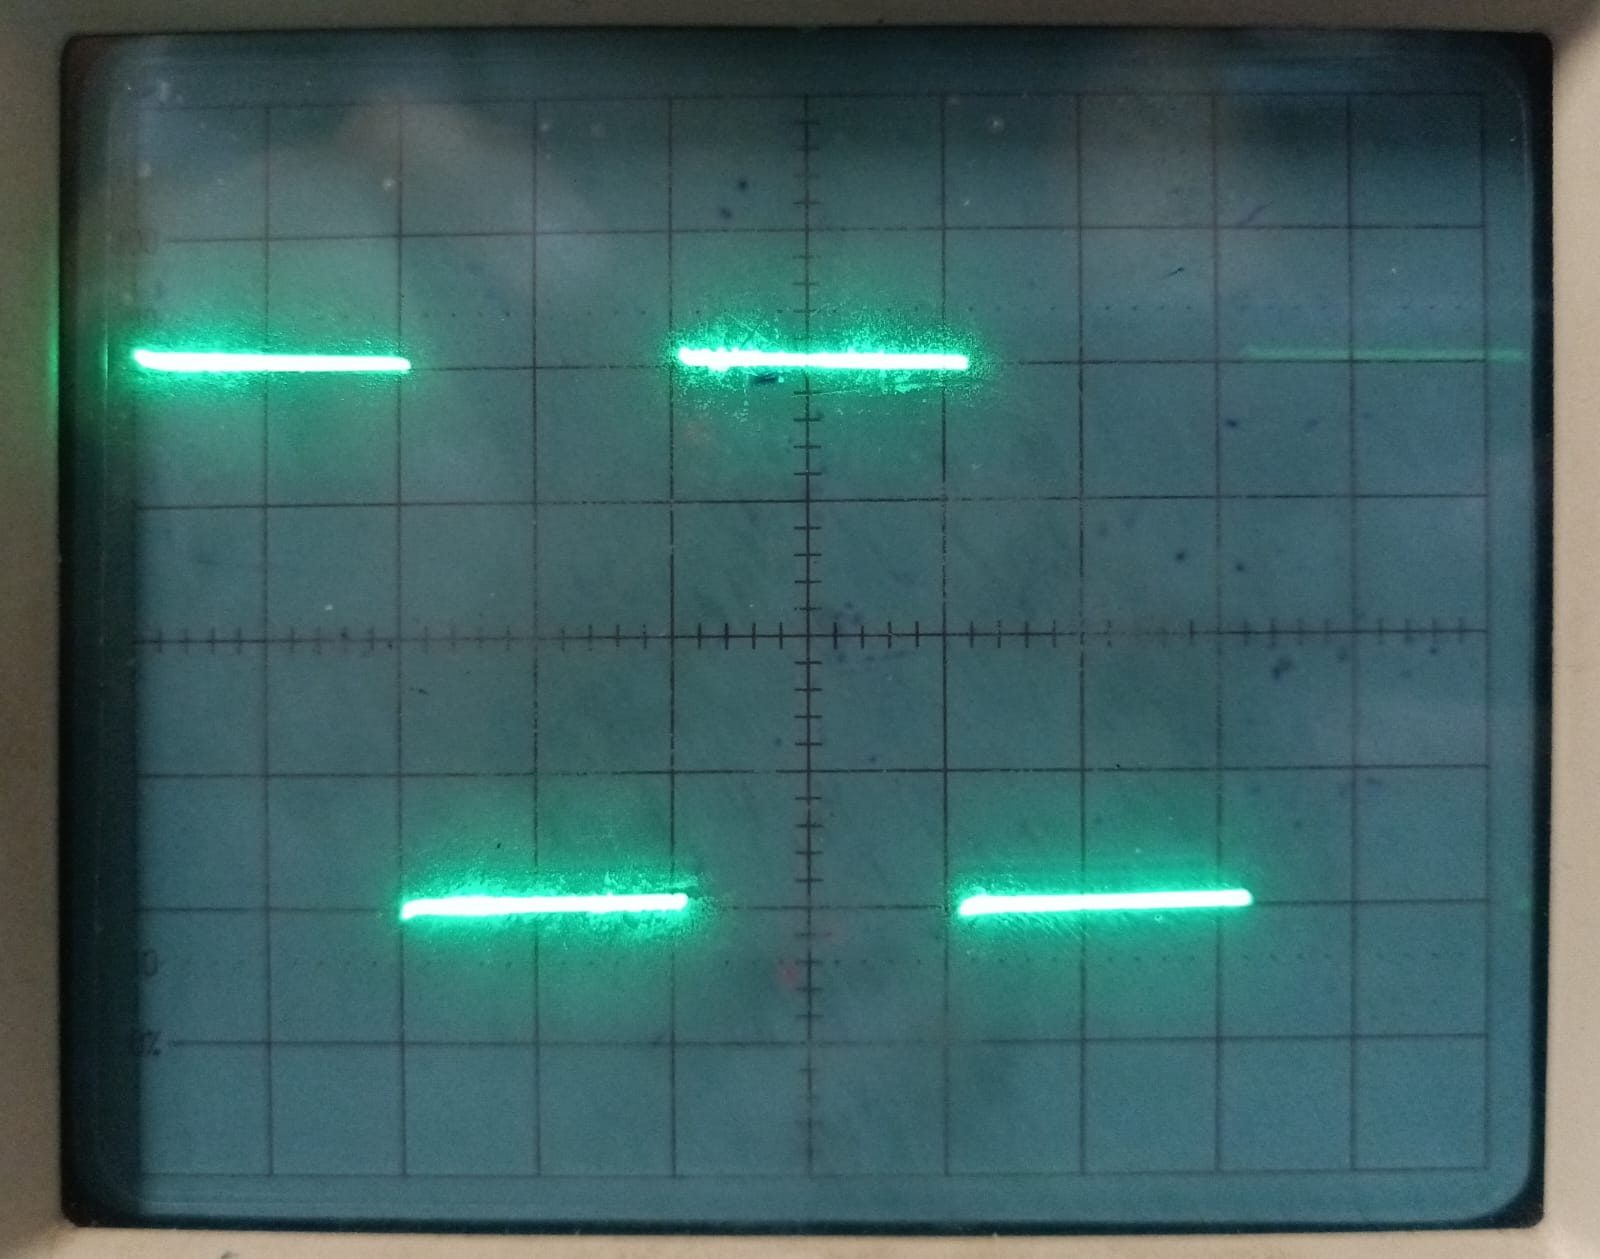
\includegraphics[width=0.77\textwidth]{Imagenes/ACx10.jpeg}
        \caption{Acoplamiento en CA}
        \label{acx10}
    \end{subfigure}
    \caption{Señal de prueba con distintos acoplamientos y punta en atenuación x10}
    \end{center}
\end{figure}

Con el acople de \textit{CC} la señal se muestra prácticamente igual que en el caso anterior también con \textit{CC}. Pero en la figura \ref{acx10}, correspondiente al acople en \textit{CA}, se puede ver que aunque siguen existiendo, las pendientes de las lineas han disminuido considerablemente (llegando al punto de casi no notarse). 
%Esto se debe a la capacitancia



\vspace{0.5cm}
\subsubsection{Midiendo Componentes de $V_{CA}$ con un osciloscopio – Disparo por “LINEA”}

Este ensayo se realiza con el objetivo de apreciar el efecto de utilizar el disparo por "LINEA" de la opción de la fuente de TRIGGER del osciloscopio, con el objetivo de visualizar de manera estable una señal o ruidos acoplados provenientes de la red eléctrica de linea.

Para ello se utilizó una fuente de baja tensión que contaba con dos salidas, una de ellas estaba regulada y marcaba 12V y la otra estaba sin regular. Luego se conectó en la salida regulada una resistencia de $39 \Omega$ ($5 W$) que será utilizada como carga. 

Si bajo estas condiciones se midiera la tensión de salida sin regular, se podrá apreciar que la señal tendrá acoplado el efecto de ripple proveniente de la etapa de filtrado previa. Es posible aproximar el valor de tensión continua de la señal si se configura el osciloscopio correctamente. El primer paso es llevar el selector de acoplamiento de entrada del canal a la
posición "GND" (entrada a masa) y ajustar la línea de base en una posición de referencia cómoda para tomar la medición. Luego se retorna el selector de acoplamiento a CC, y se configura el oscilospio para visualizar correctamente la señal.

\begin{table}[H]
    \centering
    \scalebox{1}{
    \begin{tabular}{|c|c|c|c|}
    \hline
         V/div (C. Y1) & t/div (B. tiempo) & Aten. Y1 & Disparo \\
    \hline
        0.5 $V$ & 2 $ms$ & x10 & INTERNO\\
    \hline
        \end{tabular}}
        \def\tablename{Tabla} 
        \caption{Cuadro de Controles}
        \label{tab:cont3}
\end{table}

Se conecta la punta a la salida no regulada como se observa en las figuras \ref{fig::MedSalNoRegulada1} y \ref{fig::MedSalNoRegulada2}, y se procede a calcular el voltaje multiplicando la cantidad de divisiones que se desplaza la línea sobre la pantalla por el valor de escala vertical utilizado, teniendo en cuenta que la punta se encuentra atenuada X10. El resultado de la medición fue:

$$V_{CC} = 24V$$

\begin{figure}[H]
        \begin{subfigure}[b]{0.5\textwidth}
        \centering  
        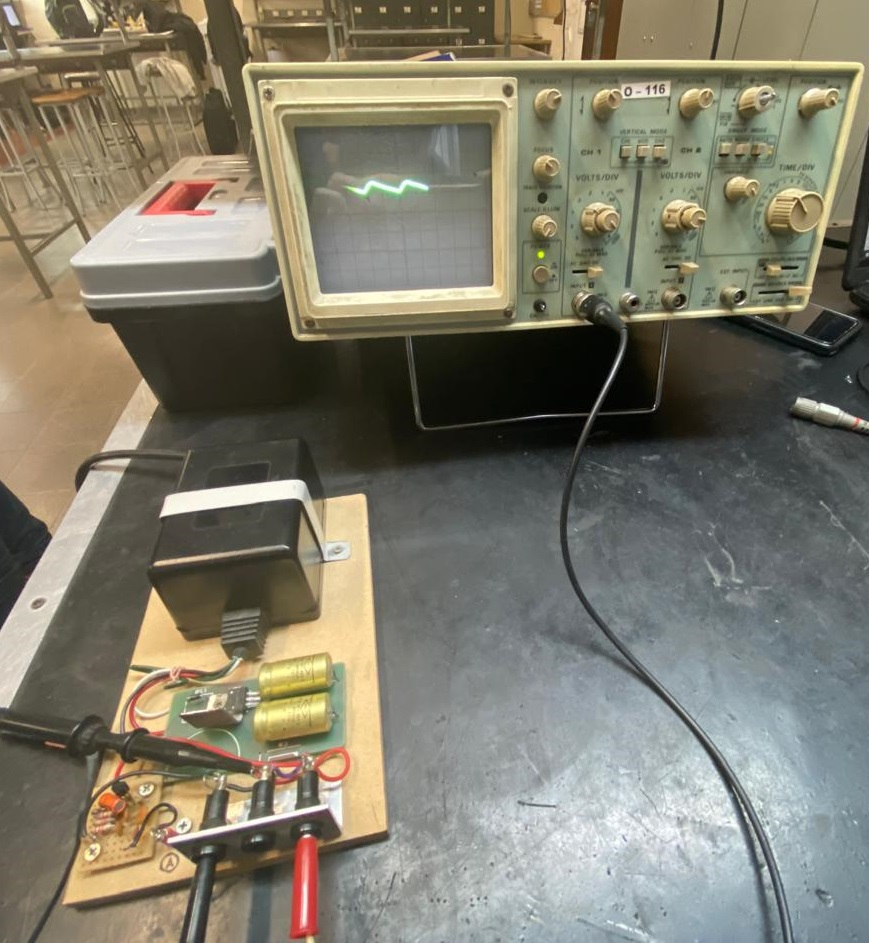
\includegraphics[width=0.85\textwidth]{Imagenes/Ensayo 3-1.jpeg}
        \caption{Medición Salida no regulada (vista 1)}
        \label{fig::MedSalNoRegulada1}
    \end{subfigure}
    \hfill
    \begin{subfigure}[b]{0.49\textwidth}
        \centering
        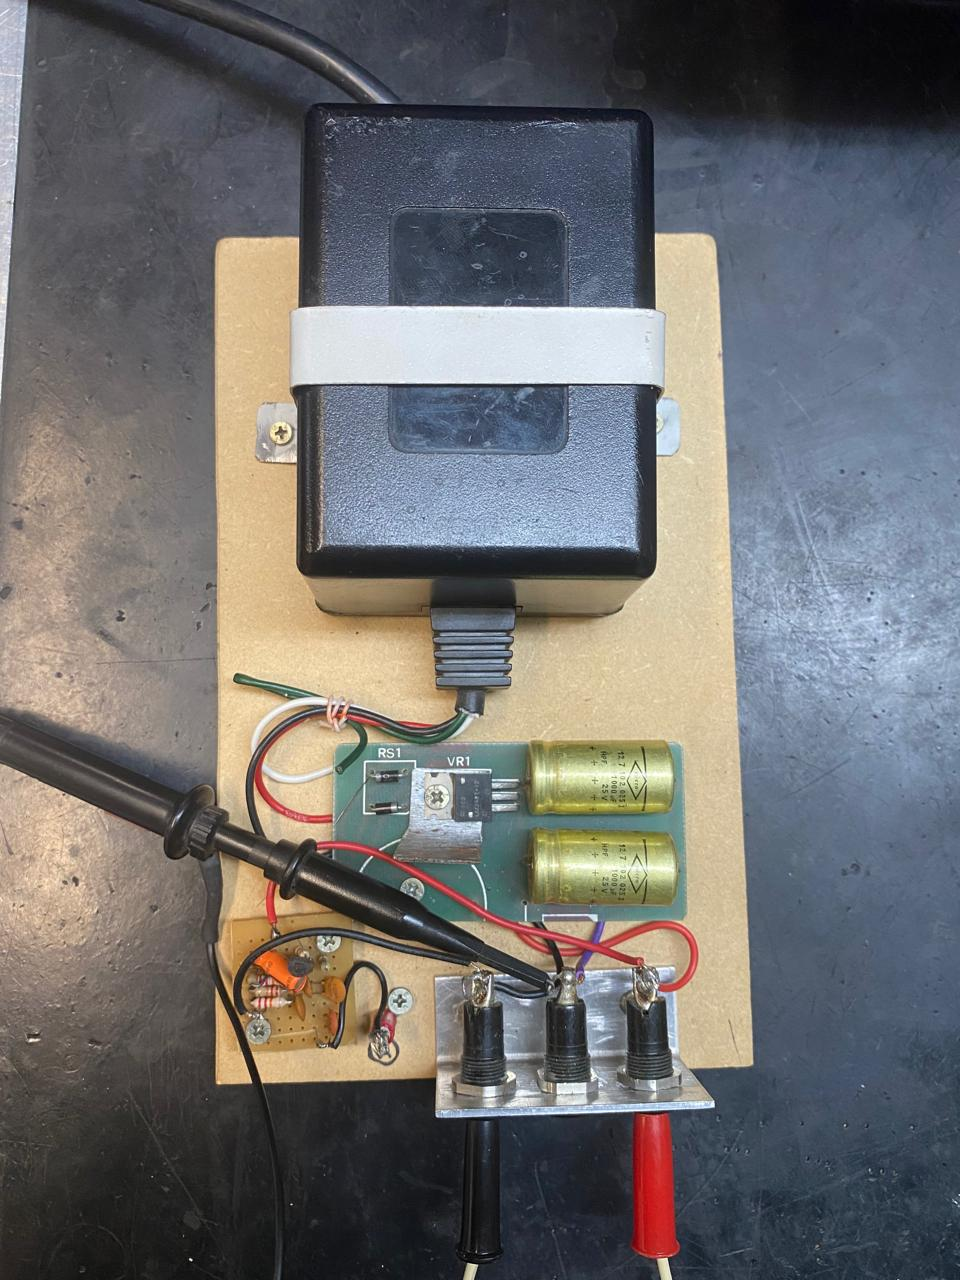
\includegraphics[width=0.7\textwidth]{Imagenes/Ensayo 3-2.jpeg}
        \caption{Medición Salida no regulada (vista 2)}
        \label{fig::MedSalNoRegulada2}
    \end{subfigure}
    \caption{Circuito de fuente regulada y no regulada, con punta en la salida no regulada}
\end{figure}


El siguiente paso del ensayo, es intentar visualizar el ripple superpuesto a la tensión de $V_{CC}$ que se está midiendo. Para ello habrá que llevar el acoplamiento a CA y se elige una configuración de escala vertical adecuada:

\begin{table}[H]
    \centering
    \scalebox{1}{
    \begin{tabular}{|c|c|c|c|}
    \hline
         V/div (C. Y1) & t/div (B. tiempo) & Aten. Y1 & Disparo \\
    \hline
        50 $mV$ & 2 $ms$ & x10 & INTERNO\\
    \hline
        \end{tabular}}
        \def\tablename{Tabla} 
        \caption{Cuadro de Controles}
        \label{tab:cont3b}
\end{table}

Se observa que el disparo está configurado en "INTERNO", lo cual produjo dificultades a la hora de ajustar el disparo. La forma correcta de realizar estas mediciones es utilizando el disparo por "LINEA", ya que la frecuencia del ruido debe ser múltiplo de la frecuencia de la tensión de línea (50 Hz). Utilizando esta nueva configuración:

\begin{table}[H]
    \centering
    \scalebox{1}{
    \begin{tabular}{|c|c|c|c|}
    \hline
         V/div (C. Y1) & t/div (B. tiempo) & Aten. Y1 & Disparo \\
    \hline
        50 $mV$ & 2 $ms$ & x10 & LINEA\\
    \hline
        \end{tabular}}
        \def\tablename{Tabla} 
        \caption{Cuadro de Controles}
        \label{tab:cont3c}
\end{table}

El valor pico a pico del ripple teniendo en cuenta la atenuación es de:

$$V_{pp_{ripple}} = 2.3V$$

En la hoja de enunciados se solicitaba completar una serie de frases sobre las características del ripple y estas quedan de la siguiente manera:

\begin{enumerate}
    \item La frecuencia del ripple superpuesto es \textit{\textbf{100}} Hz. 
    
    Esto es debido a que luego de la rectificación en el puente de diodos, queda una señal pulsante del doble de la frecuencia de la señal de entrada, en este caso la frecuencia de línea (50 Hz).
    \item El porcentaje de ripple respecto del valor de $V_{CC}$ es del \textbf{\textit{9.583}} \%.
\end{enumerate}

\begin{figure}[H]
    \centering
    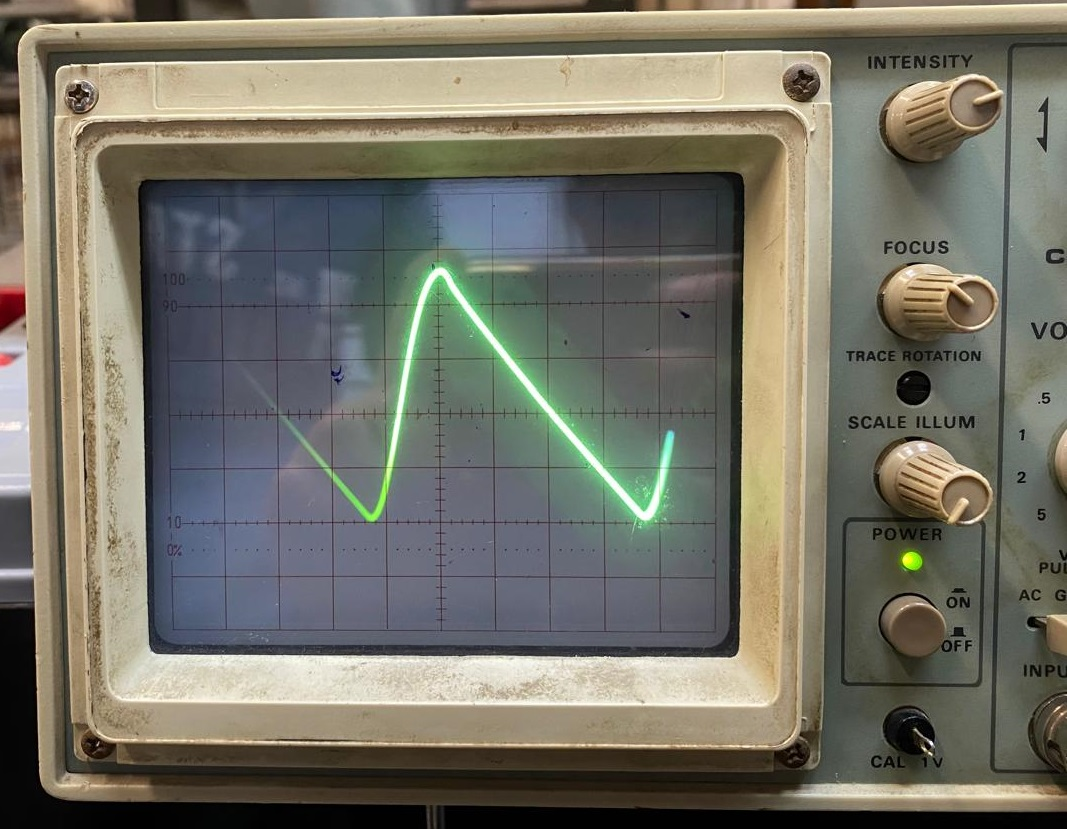
\includegraphics[width=0.6\textwidth]{Imagenes/Ensayo 3-3.jpeg}
    \caption{Medición del Ripple}
    \label{fig::MedicionRipple}
\end{figure}

\vspace{0.5cm}
\subsubsection{Usando el disparo (trigger) interno de un osciloscopio} 

Esta sección estará dedicada a comprender como funcionan algunos controles más específicos del \textit{Trigger} o disparo. En este caso, se utilizará como fuente de disparo, el trigger interno, en este caso se utilizo la señal de disparo del canal 1 (CH1).

Para comenzar, se ajustará el generador de funciones para que proporcione una onda sinusoidal, con frecuencia de 500 Hz y una amplitud de 2,5 V (Voltaje pico). 

Los parámetros para la punta y el osciloscopio serán los siguientes (tabla \ref{tab:cont4}):

\begin{table}[H]
    \centering
    \scalebox{1}{
    \begin{tabular}{|c|c|c|c|c|}
    \hline
         V/div (C. Y1) & t/div (B. tiempo) & Aten. Y1 & Acoplamiento & Disparo \\
    \hline
        0.1 $V$ & 0.5 $ms$ & x10 & CC & CH1\\
    \hline
        \end{tabular}}
        \def\tablename{Tabla} 
        \caption{Cuadro de Controles}
        \label{tab:cont4}
\end{table}

Una vez conectado el generador a la punta de osciloscopio, ponemos el selector de pendiente (\textit{slope}), en la opción "\textit{+}". Esta opción hace referencia a que el disparo se debe efectuar en algún punto de la onda donde la pendiente sea positiva. O sea que lo primero que se verá en la imagen del osciloscopio será una pendiente ascendente o positiva como en la figura \ref{fig:pendPos}.

Luego se procede a cambiar el control de pendiente a la opción "\textit{-}", lo que produce que ahora la imagen sea tomada en algún punto durante la pendiente negativa de la señal. Se ve ahora, en la figura \ref{fig:pendNeg}, que al principio de la imagen del osciloscopio la señal ahora está "bajando". 

%Este cambio de pendiente se puede pensar también como un adelanto o atraso de 90° en la señal de disparo del osciloscopio, lo que va a generar una diferencia de 90° entre las imágenes que toma mientras esta en pendiente positiva y negativa.  

%Insertar imagen de las dos pendientes subfigures

\begin{figure}[H]
        \begin{subfigure}[b]{0.5\textwidth}
        \centering  
        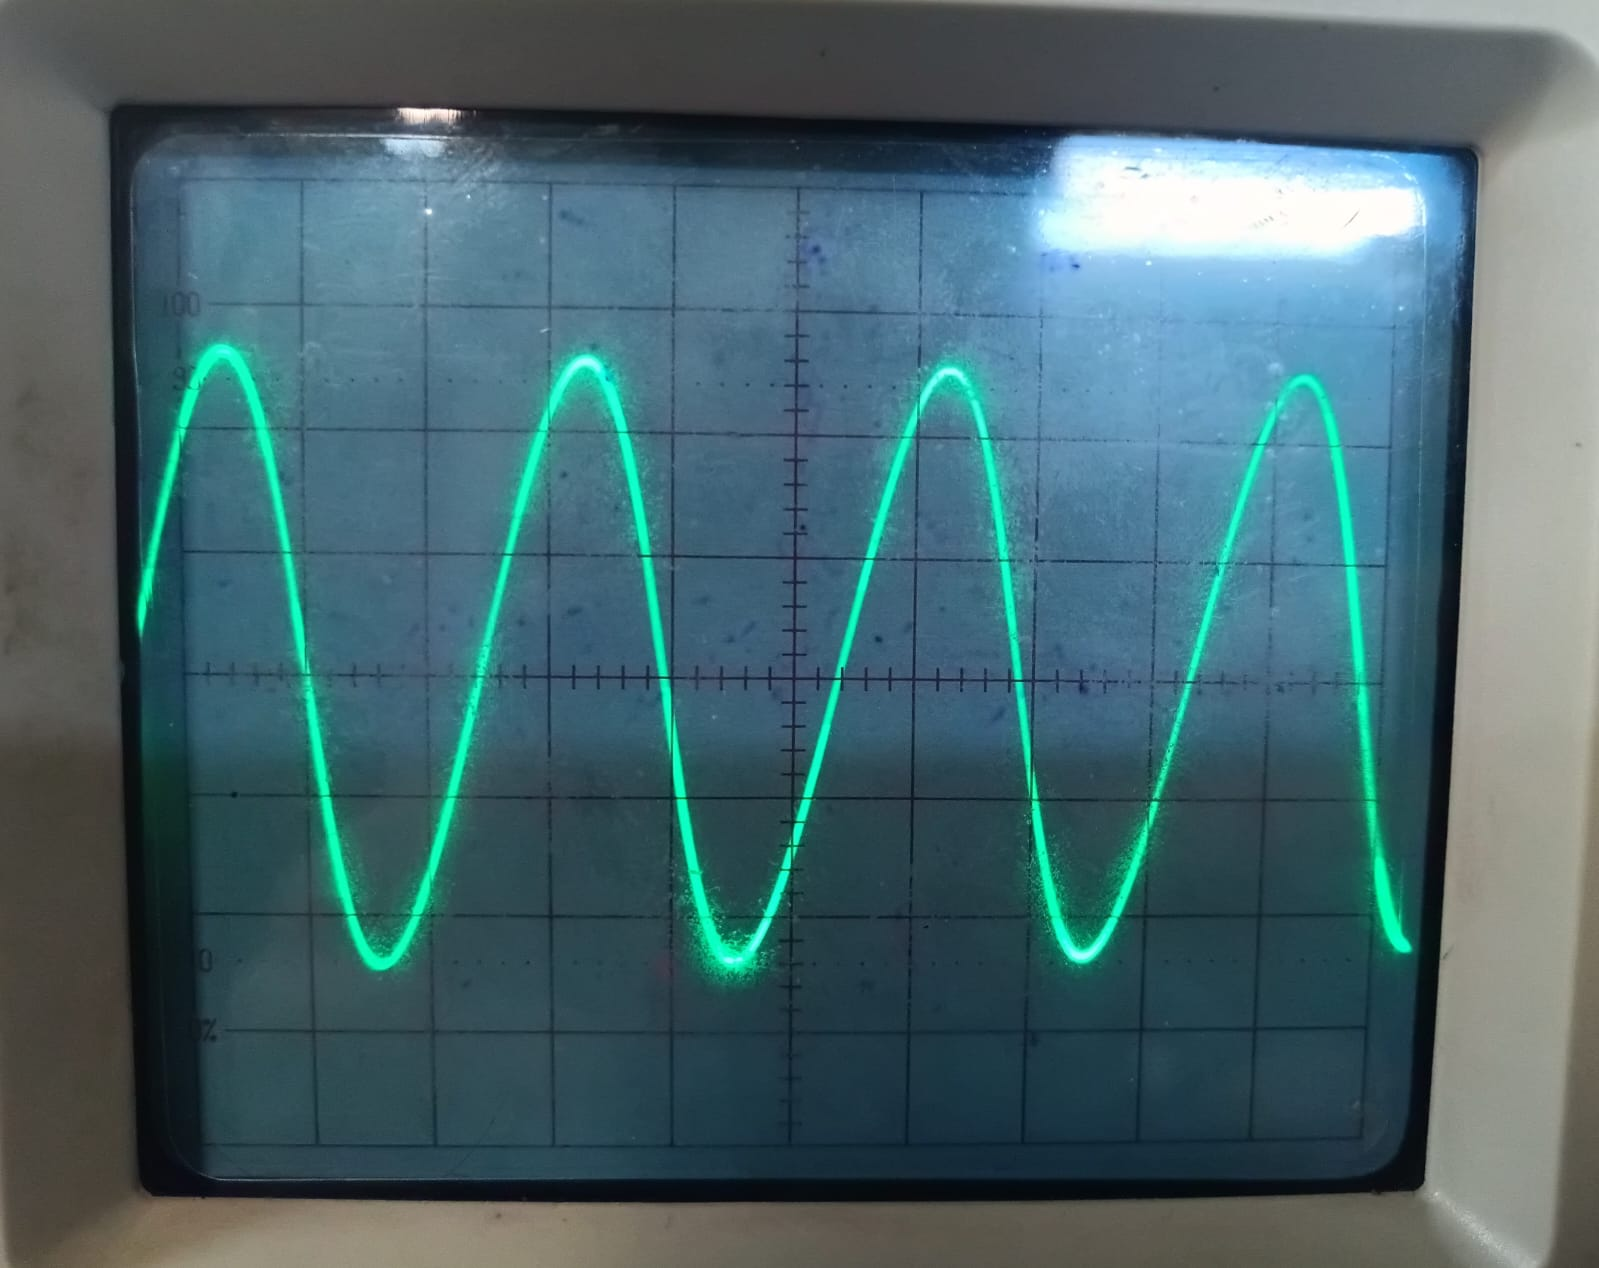
\includegraphics[width=0.85\textwidth]{Imagenes/pPos.jpeg}
        \caption{Pendiente positiva}
        \label{fig:pendPos}
    \end{subfigure}
    \hfill
    \begin{subfigure}[b]{0.49\textwidth}
        \centering
        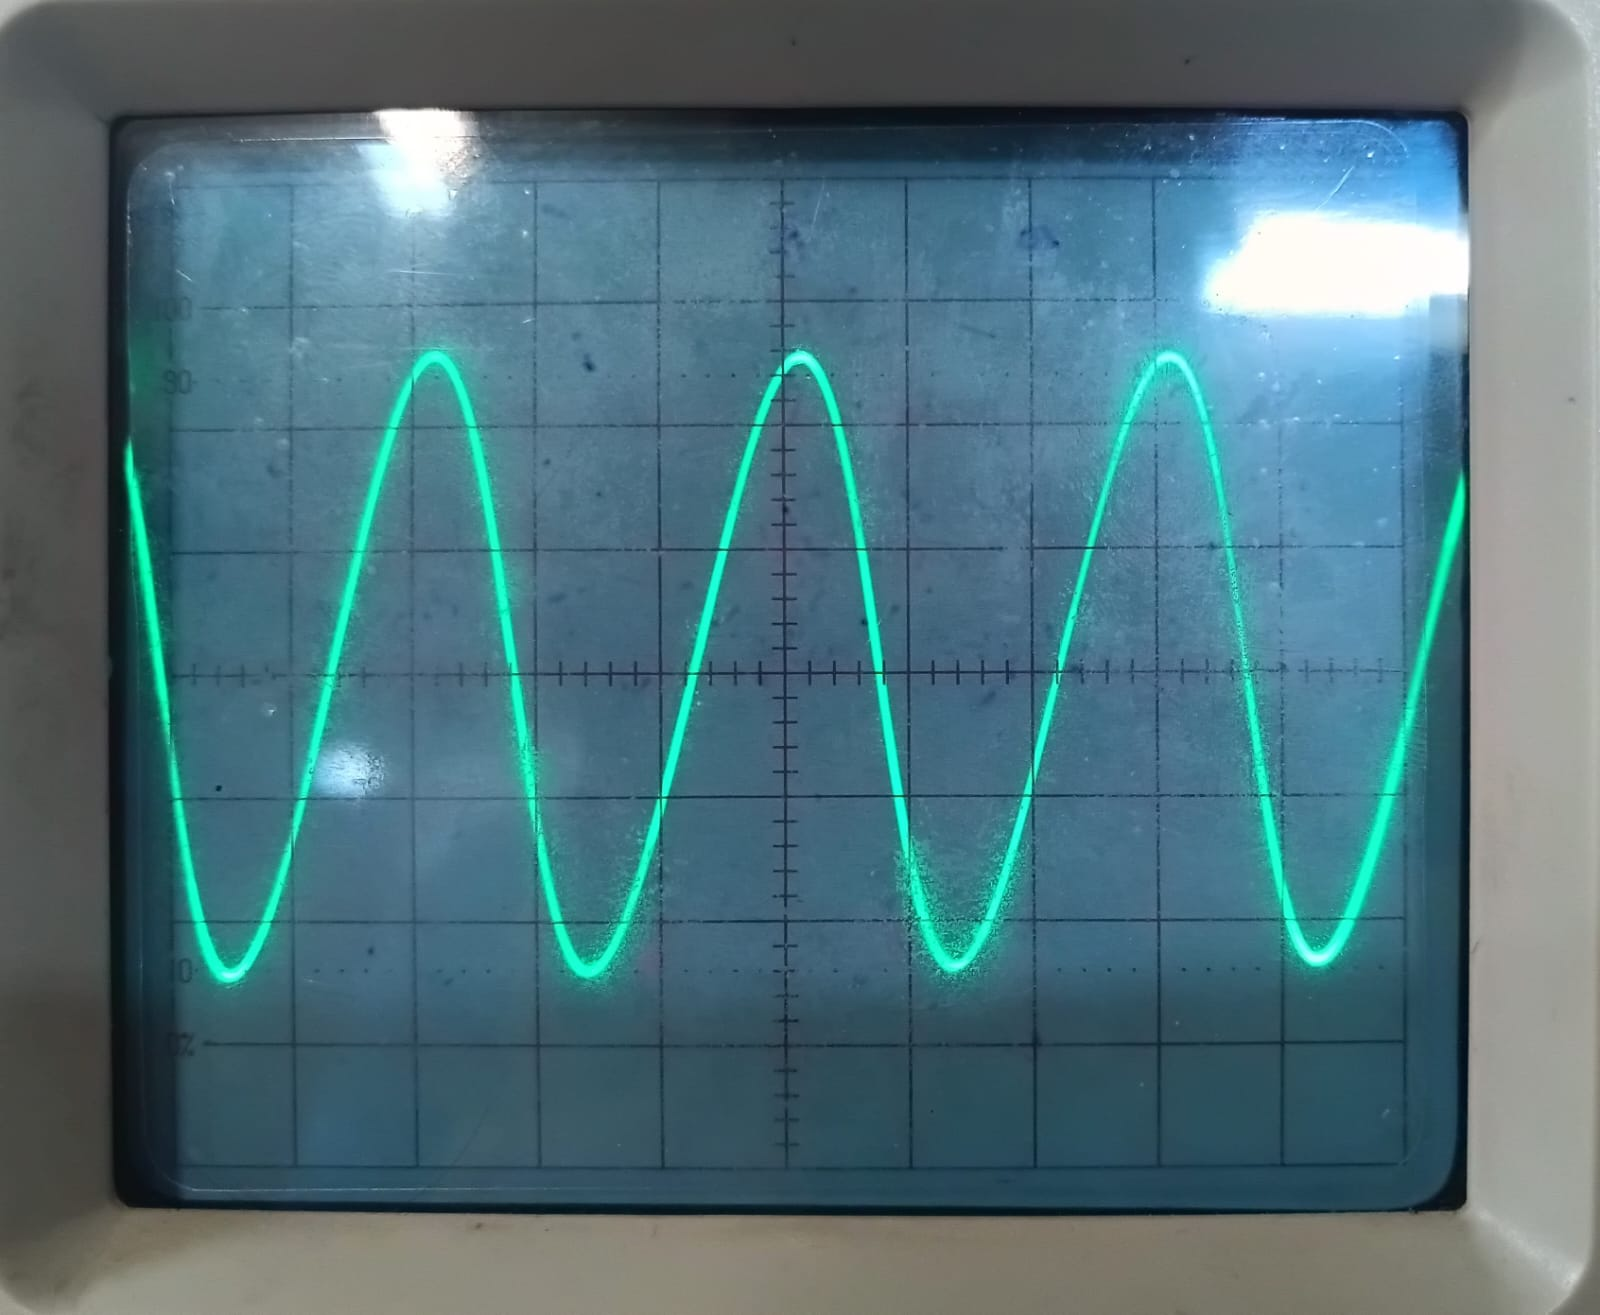
\includegraphics[width=0.85\textwidth]{Imagenes/pNeg.jpeg}
        \caption{Pendiente negativa}
        \label{fig:pendNeg}
    \end{subfigure}
    \caption{Imagen de la señal según el tipo de pendiente de disparo}
\end{figure}

Una vez comprobado el funcionamiento de la opción de pendiente, se pedía cambiar la salida del generador a onda cuadrada con una amplitud de 300 $mV_{pp}$ y ajustar la configuración del osciloscopio hasta obtener una imagen estable. 

Una vez conseguido esto, se debía reducir la amplitud de la presentación con el dial de ganancias del amplificador vertical (perilla pequeña situada sobre la perilla de sensibilidad vertical). Esta perilla regula el factor multiplicativo de entrada de la señal y va desde 1 hasta 0,33, por lo que podemos reducir la señal hasta un tercio de su valor original.

 El objetivo de modificar este elemento, era desestabilizar la señal al punto que ya no importase cuanto se modificara el nivel de disparo, para conocer cuál era el límite de sensibilidad de este. 

En esta parte encontramos complicaciones ya que la imagen podía ser estabilizada incluso con el VAR al máximo (o sea la señal al $30\%$). Para forzar la desestabilización, se debió bajar la escala de sensibilidad vertical, así logrando perder el sincronismo con la imagen (figura \ref{fig:desinc}).

%Imagen de cuando se pierde completamente el sincronismo

\begin{figure}[H]
    \centering
    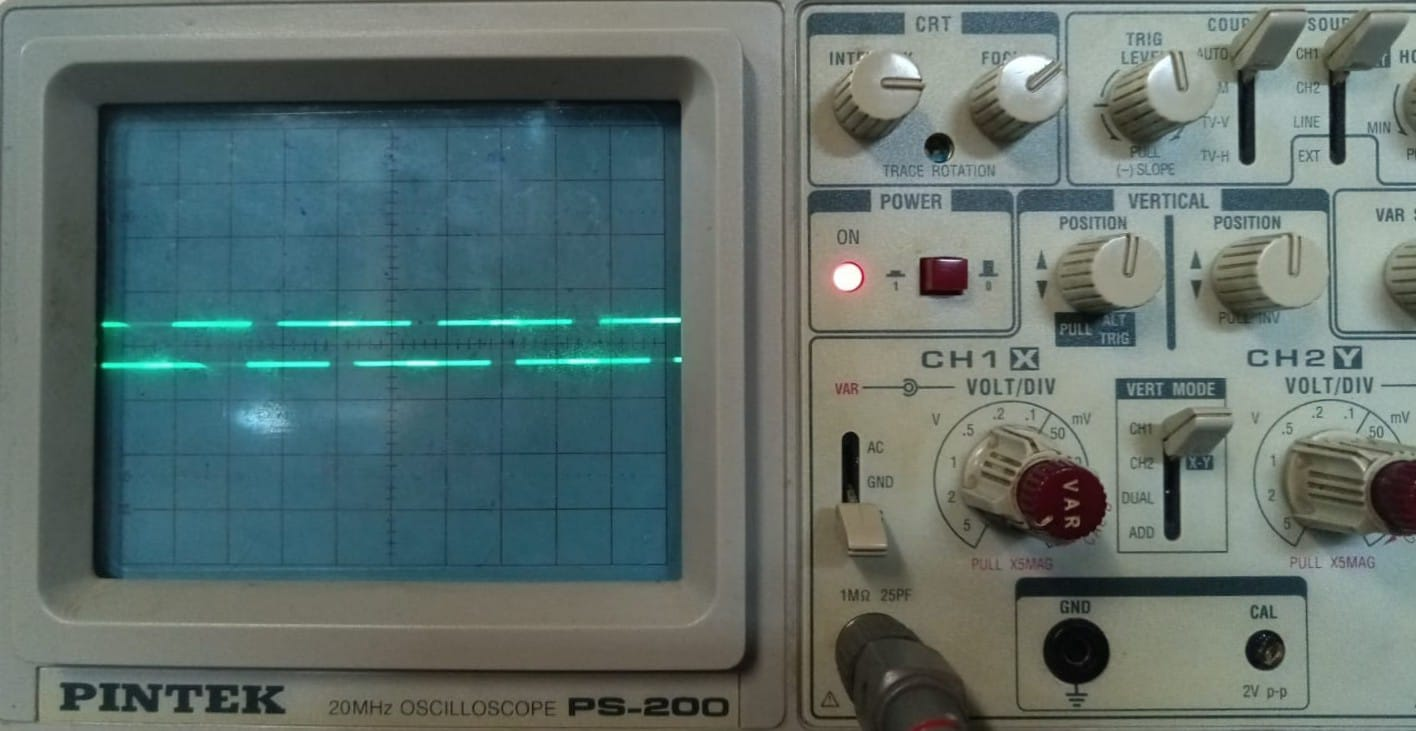
\includegraphics[width=0.8\textwidth]{Imagenes/lowTrig.jpeg}
    \caption{Señal con amplitud insuficiente para activar el circuito de disparo}
    \label{fig:desinc}
\end{figure}

A partir de esto, se pudo ver que:

\begin{itemize}
    \item El nivel mínimo de señal que activa el circuito de trigger es de \textit{\textbf{0.5}} divisiones de la pantalla.
\end{itemize}

\vspace{0.5cm}
\subsubsection{Usando el disparo externo de un osciloscopio}

Este ensayo tiene como finalidad descubrir una de las múltiples y variadas aplicaciones que tiene el trigger o disparo externo del osciloscopio 

Para ello, se dejo la configuración del ensayo anterior. Se conecto la entrada de "trigger externo" del osciloscopio a la salida "SYNC" del generador de funciones. Esta es una salida de una señal de disparo rectangular de la misma frecuencia que la señal de la salida principal. Luego se cambio la fuente de disparo de la base de tiempos a "Externo" y se ajusto el nivel de disparo hasta que se obtuvo una imagen estable de la señal.

Como siguiente paso, se fue variando el nivel de la señal y cambiando la sensibilidad vertical (V/div), y aquí pudimos observar que, gracias al uso del disparo externo, la imagen nunca perdía sincronismo y se mantuvo estable.

\begin{figure}[H]
        \begin{subfigure}[b]{0.5\textwidth}
        \centering  
        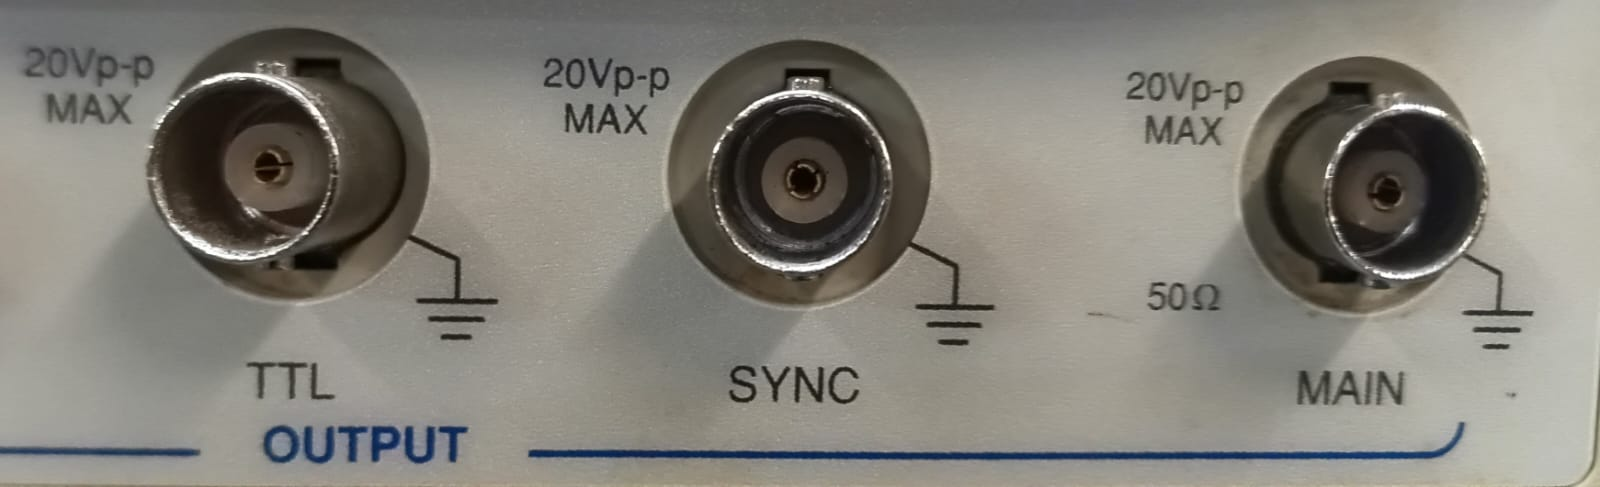
\includegraphics[width=0.85\textwidth]{Imagenes/SYNC.jpeg}
        \caption{Salida de sincronización (SYNC) del generador}
        \label{fig:SYNC}
    \end{subfigure}
    \hfill
    \begin{subfigure}[b]{0.49\textwidth}
        \centering
        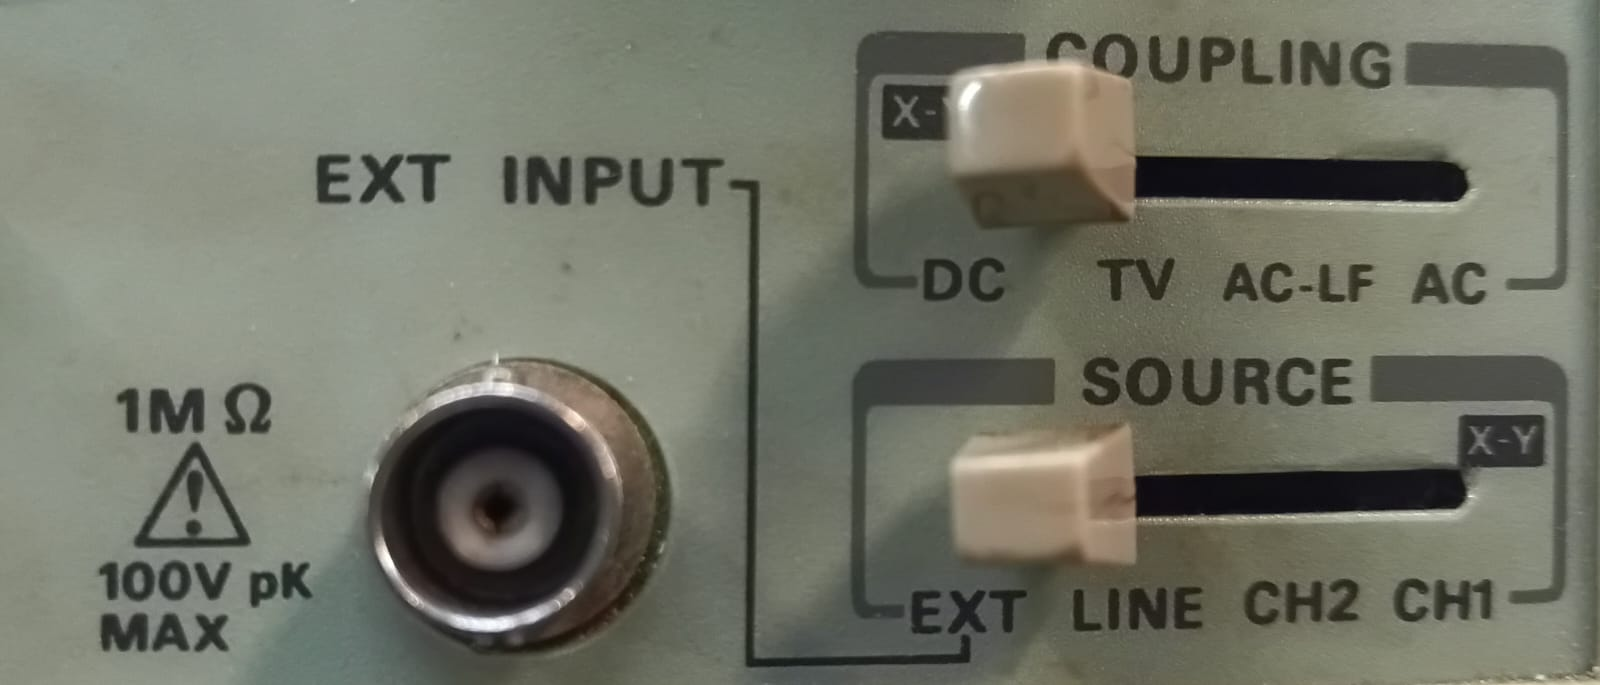
\includegraphics[width=0.7\textwidth]{Imagenes/EXT.jpeg}
        \caption{Entrada del pulso externo de disparo del osciloscopio}
        \label{fig:EXT}
    \end{subfigure}
    \caption{Conectores de la salida de sincronización}
\end{figure}


\vspace{0.5cm}
\subsubsection{Usando el modo X-Y para medir frecuencia por comparación con la salida de un
generador de referencia (figura de Lissajous)}

En este ensayo se verá la utilidad del modo X-Y para la medición de la frecuencia de una
determinada señal que proviene de un generador "A" sin visor. Se puede estimar que su “frecuencia nominal” de salida es aproximadamente a 400 Hz, pero se se desea encontrar su valor exacto.

Para ello, se utilizó como referencia la señal producida por el generador de funciones \textit{GFG 3015 (B)}, que tiene un visor digital que indica la frecuencia.

El primer paso fue conectar la señal del generador A en el canal 1, y utilizando el disparo "INTERNO" se configuró el osciloscopio para poder visualizar la señal y medir su amplitud:

\begin{table}[H]
    \centering
    \scalebox{1}{
    \begin{tabular}{|c|c|c|c|}
    \hline
         Frec. (nominal) & Forma de onda & Ampl. (pico a pico) \\
    \hline
        400 Hz & Sinusoidal & 0.8 V \\
    \hline
        \end{tabular}}
        \def\tablename{Tabla} 
        \caption{Cuadro de Controles}
        \label{tab:cont6}
\end{table}

Luego se conectó la salida del generador GFG
3015 al canal 2 del osciloscopio. La forma de la señal de salida es también sinusoidal, y se configuró su amplitud al mismo valor que la señal del canal 1. Como el valor de frecuencia de la señal del generador A se estima en 400 Hz, se configura como frecuencia inicial del generador GFG 3015 a 400 Hz.

El siguiente paso fue activar el modo X-Y del osciloscopio con el objetivo de visualizar las figuras de Lissajous. Como las frecuencias de ambas señales no coincidieron al primer intento, se tuvo que modificar el valor de la frecuencia del generador GFG 3015 hasta que se pudo visualizar la forma de una elipse en el visor del osciloscopio, como se observa en la figura \ref{fig::Lissajou}. La frecuencia del generador A medida entonces fue de:

$$Frecuencia = 372.01 Hz$$

Es importante aclarar que si las señales de ambos canales estuvieran en fase (además de tener la misma frecuencia y amplitud), la figura de Lissajou debería aproximarse más a una línea, sin embargo, como existía cierto desfase en nuestras señales, la figura observada es una elipse. Si el desfase entre las señales fuera de exactamente 90°, en la imagen se vería un circulo perfecto.

\begin{figure}[H]
    \centering
        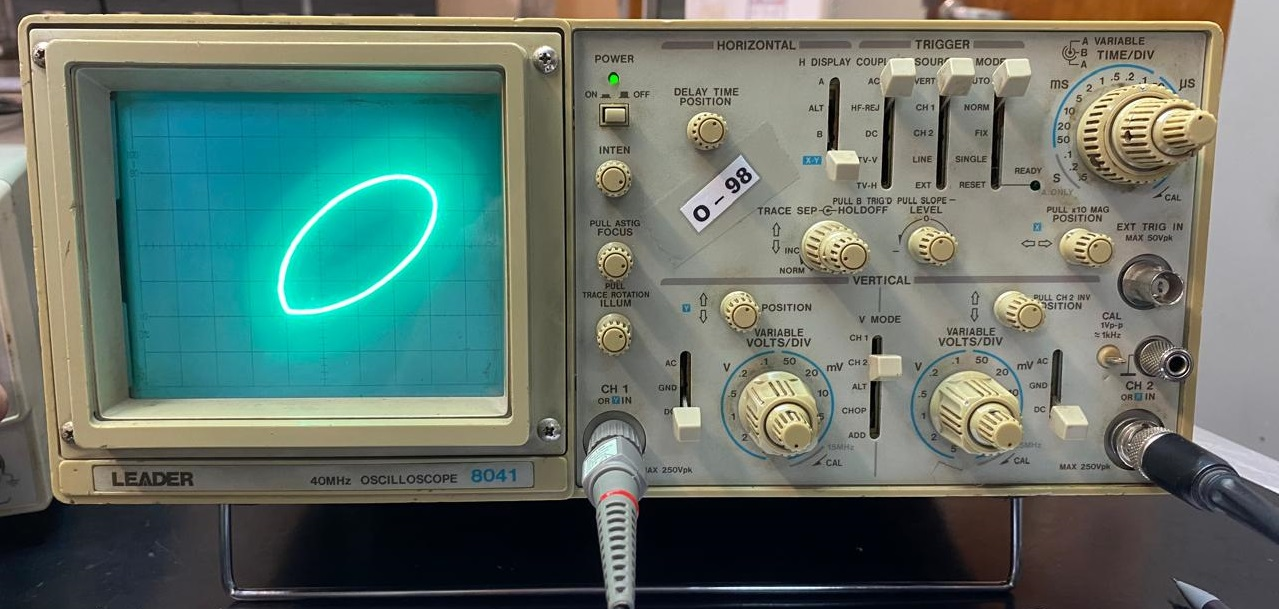
\includegraphics[width=0.8\textwidth]{Imagenes/Ensayo 6.jpeg}
    \caption{Figura de Lissajou}
    \label{fig::Lissajou}
\end{figure}


\vspace{0.5cm}
\subsubsection{Usando el Hold-off}

En esta parte del trabajo se emplea nuevamente el generador GFG 3015 para obtener una forma de
onda específica. Para ello debe disponer los controles del mismo de la siguiente manera (tabla \ref{tab:cont7}):

\begin{table}[H]
    \centering
    \scalebox{0.85}{
    \begin{tabular}%{|c|c|c|c|c|c|c|c|c|c|c|c|}
    {|c|m{1.3cm}|m{1.6cm}|m{1.2cm}|m{1.6cm}|m{1.3cm}|m{1.5cm}|m{1.2cm}|m{1.2cm}|m{1.5cm}|m{1.5cm}|m{1.3cm}|}
    \hline
         $f$ & Func. & Ampl. & Duty & Trig. Mult/Sing & Trig. Ext. & Rate & Sym & Trig. Phase & Shift + Source & Trig. on/off \\
    \hline
        2 kHz & Cuadr. & 5 $V_{pp}$ & 50 \% & Mult. & Desact. & 0.5 KHz & 50\% & 30\% & Triang. & on \\
    \hline
        \end{tabular}}
        \def\tablename{Tabla} 
        \caption{Disposición de controles del generador}
        \label{tab:gen7}
\end{table}


Bajo estas condiciones, la señal de salida esperada debería tener la forma de la figura \ref{fig::TrenDePulsosEsperado}. 

\begin{figure}[H]
    \centering
        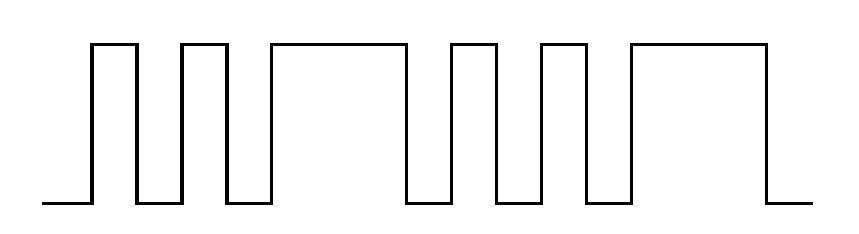
\includegraphics[width=0.7\textwidth]{Imagenes/Ensayo 7 - tren ideal.png}
    \caption{Tren de pulsos esperado}
    \label{fig::TrenDePulsosEsperado}
\end{figure}

Para verificarlo, se conecta la señal al canal 1 del osciloscopio. Se dispone del disparo "INTERNO" (canal 1), y a pesar de tener la base del tiempo correctamente configurada, la señal visualizada en el instrumento se encuentra distorsionada. Se observa claramente una superposición de dos imágenes. Esto es debido a que el disparo interno del osciloscopio no distingue entre los flanco del pulso ancho y el delgado, por lo que el disparo no se lleva a cabo. En esta situación mover el nivel del trigger no tendría efecto alguno para solucionar el problema.

Para poder visualizar correctamente el tren de pulsos, se debe configurar el valor de \textit{Hold-off}. Mediante este parámetro se puede establecer un retardo al disparo, y de esa forma omitir el flanco del pulso ancho, y realizar el disparo siempre en la misma porción de la señal.

Regulando entonces el control de \textit{Hold-off}, la señal visualizada sin interferencias se puede apreciar en la figura \ref{fig::TrenDePulsosOsc}.

\begin{table}[H]
    \centering
    \scalebox{1}{
    \begin{tabular}{|c|c|c|c|}
    \hline
         V/div (C. Y1) & t/div (B. tiempo) & Aten. Y1 & Disparo \\
    \hline
        .2V $V$ & 0.2 $ms$ & x10 & INT \\
    \hline
        \end{tabular}}
        \def\tablename{Tabla} 
        \caption{Cuadro de Controles}
        \label{tab:cont7}
\end{table}

\begin{figure}[H]
    \centering
        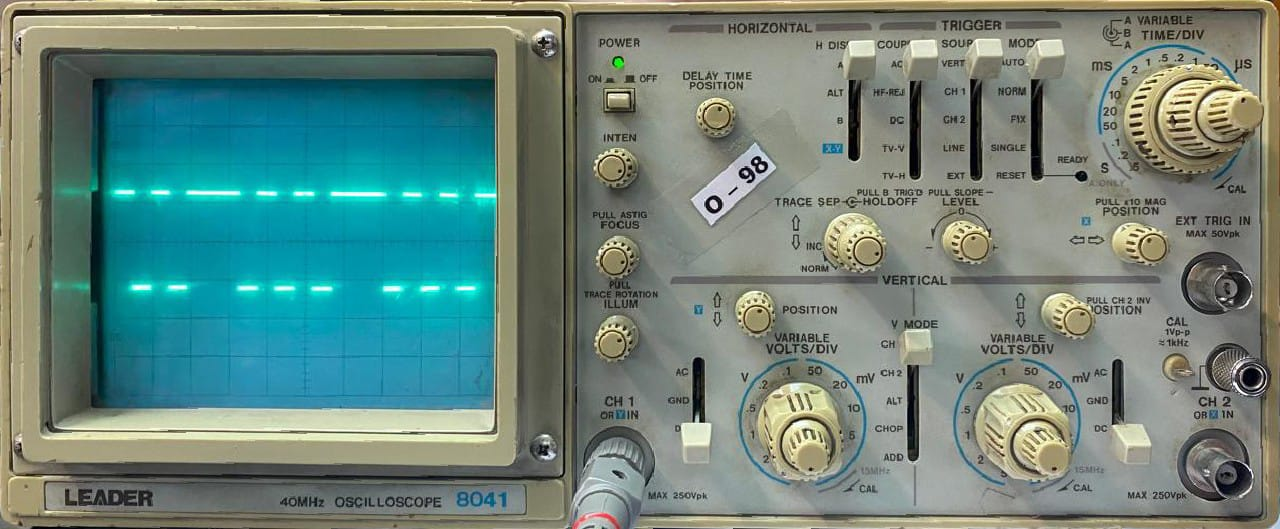
\includegraphics[width=\textwidth]{Imagenes/holdoff.jpeg}
    \caption{Tren de pulsos de diversos anchos en osciloscopio}
\label{fig::TrenDePulsosOsc}
\end{figure}


\vspace{0.5cm}
\subsubsection{Usando el Doble Trazo}

Este experimento se realizó con el objetivo de utilizar la función de doble trazo del osciloscopio para poder observar la relación existente entre dos señales.

Partiendo del ensayo anterior, se conecta el canal 2 a la salida del generador GFG 3015 identificada con el rótulo MOD. Se procede a activar el doble trazo en modo “ALTERNADO” para visualizar ambos canales, y se ajusta la sensibilidad vertical del canal 2 para obtener una imagen adecuada.

\begin{table}[H]
    \scalebox{1}{
    \begin{tabular}{|c|c|c|c|c|c|c|}
    \hline
         V/div (C. Y1) & V/div (C.Y2) & t/div & Aten. Y1 & Aten. Y2 & Acop.(Y1/Y2) & Disparo \\
    \hline
        50 $mV$ & 1 $V$ & 0.1 $ms$ & x10 & x10 & CC & ALT\\
    \hline
    \end{tabular}}
        %\def\tablename{Tabla} 
        \caption{Cuadro de Controles}
        \label{tab:cont8}
\end{table}



Se observa en la figura \ref{fig::TrenDePulsosDobleTrazo} que la señal del canal 2 es de forma triangular simple, y su período coincide con el período de la señal previamente configurada en el canal 1. 

Analizando esta relación se llega a la conclusión de que si establecemos el disparo interno en el canal 2, será mucho más sencillo estabilizar la imagen del canal 1, sin necesidad de recurrir al control de \textit{Hold-off}.

\begin{figure}[H]
    \centering
        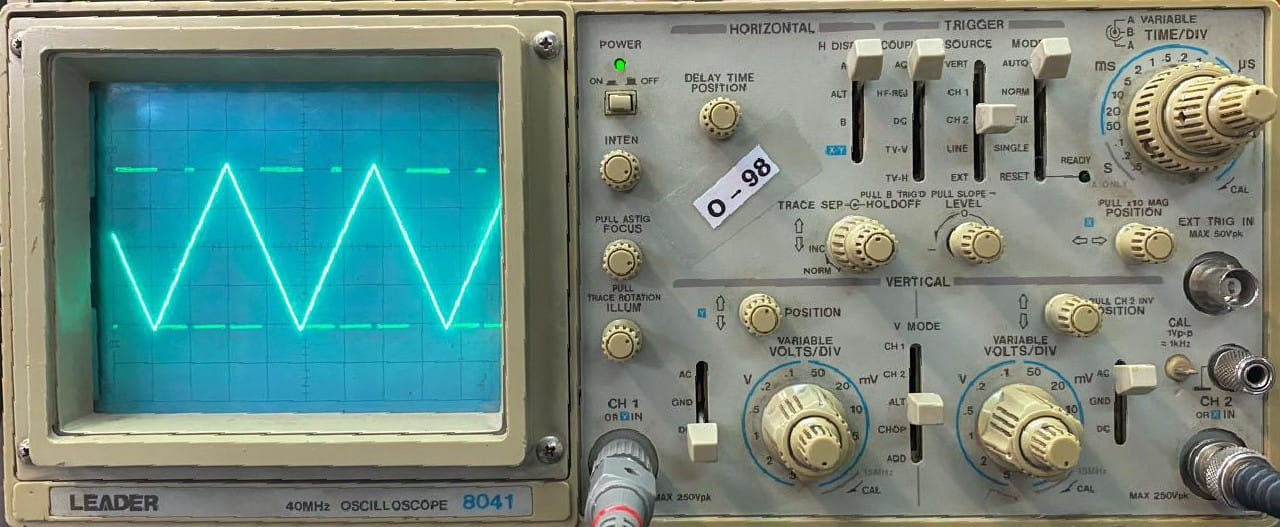
\includegraphics[width=0.8\textwidth]{Imagenes/exp8.jpeg}
    \caption{Usando el Doble Trazo}
    \label{fig::TrenDePulsosDobleTrazo}
\end{figure}

Como se puede apreciar en la figura\ref{fig::TrenDePulsosDobleTrazo} la señal tanto del canal 1 como del canal 2, tienen el mismo periodo el cual es de $0.4ms$, también las señales están en fase. Las amplitudes medidas a través del osciloscopio serian de $5V_{pp}$ para la señal de pulsos y $2V_{pp}$ para la señal triangular. 

A continuación se presenta un gráfico en grilla de las señales de ambos canales. La escala vertical es de 0.75V por división, y la escala horizontal es de 50 $\mu s$ por división.

\begin{figure}[H]
    \centering
        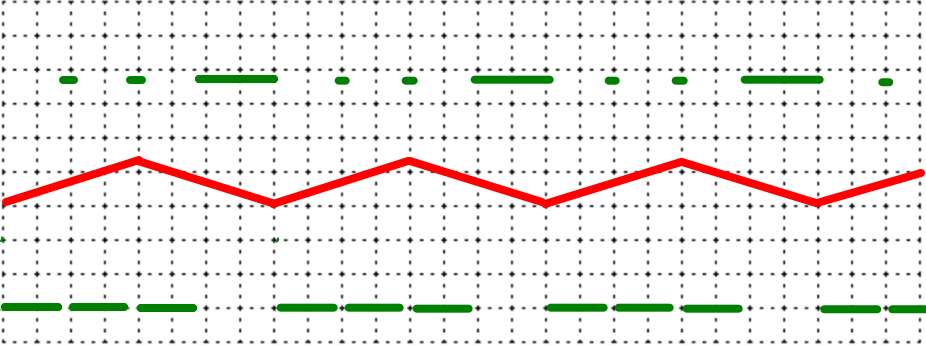
\includegraphics[width=1\textwidth]{Imagenes/Grilla ensayo 8.png}
    \caption{Gráfico a escala de ambas señales.}
\label{fig::TrenDePulsosOsc}
\end{figure}

%%%%%%%%%%%%%%%%%%%%%%%%%%%%%%%%%%%%%5   puto el que lee
%%%%%%%%%%%%%%%%%%%%%%%%%%%%%%%%%%%%%%%%%%%%%%%%%%%%%%%%%%%%%%%%%%%%%%%%%%
% Falta: la correspondencia temporal entre las dos señales(xd no se que es esto  )

% Falta poner el << Cuadro de controles >>, no lo puse porque no entiendo las configuracions que se ven en la foto
%%%%%%%%%%%%%%%%%%%%%%%%%%%%%%%%%%%%%%%%%%%%%%%%%%%%%%%%%%%%%%%%%%%%%%%%%%

\vspace{0.5cm}
\subsubsection{Empleo de los filtros de rechazo de la sección de disparo de la base de tiempos}
El objetivo de esta experimentación es comprender el uso y aplicación de los filtros de rechazo TV-H y TV-V, de la sección de disparos de la base de tiempos.

Para ello se configuro el generador de funciones GFG 3015 de la siguiente manera:

\begin{table}[H]
    \centering
    \scalebox{0.85}{
    \begin{tabular}%{|c|c|c|c|c|c|c|c|c|c|c|c|}
    {|m{1.7cm}|m{1.3cm}|m{1.6cm}|m{1.2cm}|m{1.6cm}|m{1.3cm}|m{1.5cm}|m{1.2cm}|m{1.2cm}|m{1.3cm}|m{1.5cm}|m{1.2cm}|}
    \hline
         Frec. & Func. & Ampl. & Duty & Trig. Mult/Sing & Trig. Ext. & Rate & Sym & Trig. Phase & Shift + Source & Trig. on/off \\
    \hline
        15,6 kHz & Sen. & 5 $V_{pp}$ & 50 \% & Mult. & Desact. & 50 Hz & 50\% & 30\% & Triang. & on \\
    \hline
        \end{tabular}}
        \def\tablename{Tabla} 
        \caption{Disposición de controles del generador}
        \label{tab:gen9}
\end{table}

Esta configuración debería generar una señal con la siguiente forma:

\begin{figure}[H]
    \centering
        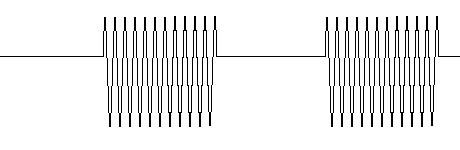
\includegraphics[width=0.7\textwidth]{Imagenes/onda_tv.png}
    \caption{Ráfaga de señal sinusoidal}
\label{fig::TrenDePulsosOsc}
\end{figure}

Esta es una señal formada por paquetes o ráfagas de de una onda sinusoidal de 15,6 kHz similar por lo menos en lo que respecta a las frecuencias, a una señal compuesta de vídeo de televisión analógica.

Para poder observar esta señal en el osciloscopio analógico, en principio, se ajusto la base de tiempos a 5ms/div y la sensibilidad vertical a 0.2V/div, y con el disparo de la base de tiempo en "interno" se intento estabilizar la imagen, pero esto no se pudo lograr. Por lo tanto se procedió a usar el filtro TV-V, con el cual fue mucho mas sencillo estabilizar y observar la imagen de salida del generador.

\begin{figure}[H]
    \centering
        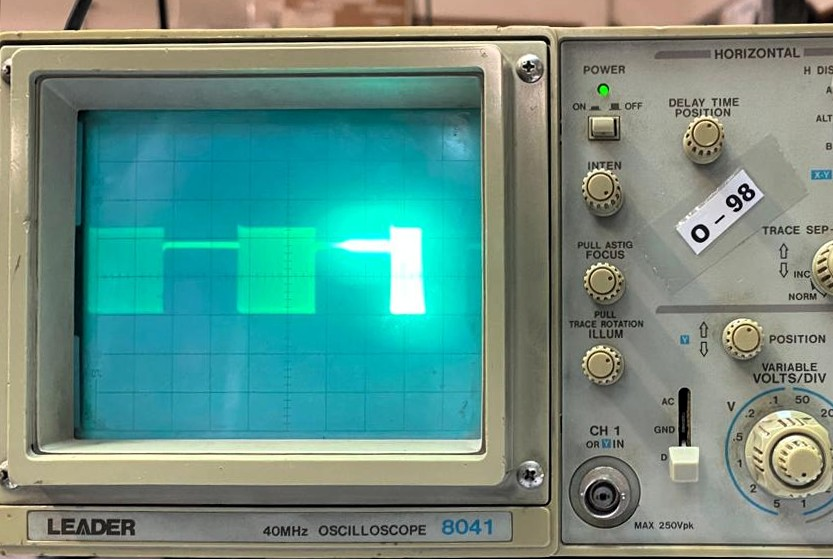
\includegraphics[width=0.6\textwidth]{Imagenes/WhatsApp Image 2024-04-25 at 10.08.42.jpeg}
    \caption{Ráfaga de señal sinusoidal vista en osciloscopio}
\label{fig::TrenDePulsosOsc}
\end{figure}

Esta imagen se pudo ver gracias a que el filtro TV-V, ajusta la respuesta del osciloscopio a la frecuencia vertical de una señal de vídeo estándar, garantizando que este pueda mostrar correctamente la forma de onda de la señal de vídeo y sincronizar las señales verticales para obtener una representación visual precisa. 

Luego, sin modificar ningún otro control se llevo la base de tiempos a 50 $\mu$S y se cambio al filtro TV-H. Esto hizo que ahora en la pantalla se pueda observar la señal de 15,6 kHz.

\begin{figure}[H]
    \centering
        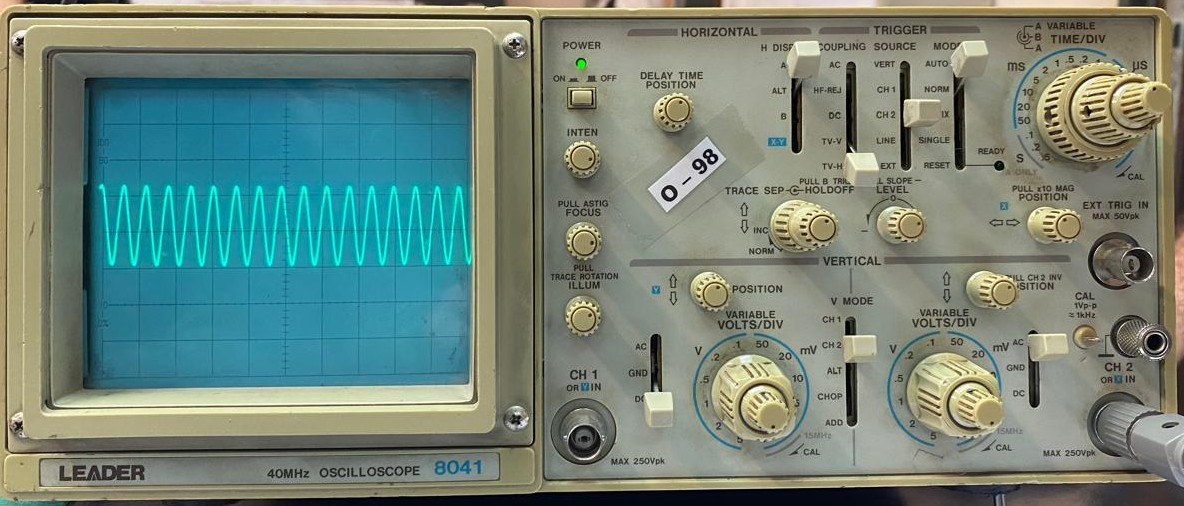
\includegraphics[width=0.8\textwidth]{Imagenes/frec_TV-H.jpeg}
    \caption{Onda sinusoidal de 15,6 kHz}
\label{fig::TrenDePulsosOsc}
\end{figure}

Nuevamente, la imagen de esta onda se pudo ver estable y precisa, gracias al filtro TV-H, ya que este se encarga de ajustar la respuesta del osciloscopio, tomando como referencia la frecuencia horizontal de una señal de vídeo estándar 

\vspace{0.5cm}
\subsubsection{Utilizando la función “Suma + Canal Invertido” de un osciloscopio – Medición del valor eficaz de un tren de pulsos}
Para esta experimentación se utilizo el generador de funciones configurado de la siguiente manera (tabla \ref{tab:gen10}):

\begin{table}[H]
    \centering
    \scalebox{1}{
    \begin{tabular}{|c|c|c|c|c|c|}
    \hline
         $f$ & Func. & Ampl. & Duty & Trig. on/off \\
    \hline
        1 kHz & Cuadr. & 10 $V_{pp}$ & 20 \% & off \\
    \hline
        \end{tabular}}
        \def\tablename{Tabla} 
        \caption{Disposición de controles del generador para experimento 10}
        \label{tab:gen10}
\end{table}
A la salida del generador se conecta un circuito auxiliar cuya única función es producir una señal de salida tipo “tren de pulsos” diferencial.

\begin{figure}[H]
        \begin{subfigure}[b]{0.6\textwidth}
        \centering  
        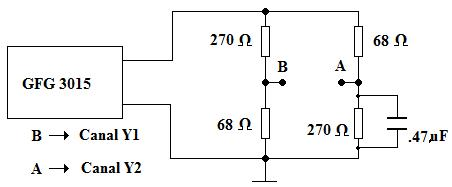
\includegraphics[width=1\textwidth]{Imagenes/circ_aux10.jpg}
        \caption{Esquemático}
        \label{fig:esqCirc10}
    \end{subfigure}
    \hfill
    \begin{subfigure}[b]{0.4\textwidth}
        \centering
        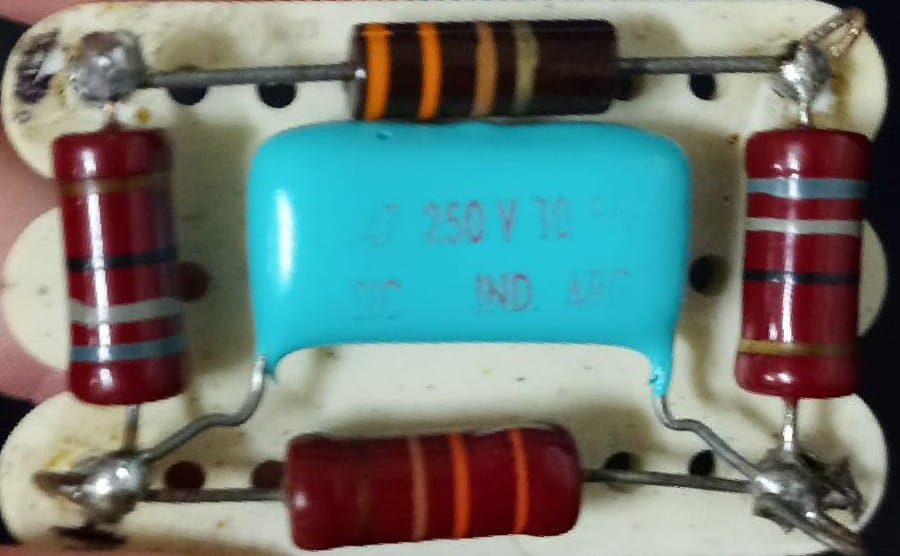
\includegraphics[width=0.7\textwidth]{Imagenes/circ10.jpeg}
        \caption{Circuito Real}
        \label{fig:placa10}
    \end{subfigure}
    \caption{Circuito con salida diferencial}
    \label{fig::CircAux10}
\end{figure}

El punto de conexión \textit{A} es el nodo inferior derecho de la figura \ref{fig:placa10} (punto), el punto \textit{B} es el de la esquina superior izquierda, el punto de conexión a masa es la esquina inferior izquierda y por último el positivo es el de la esquina superior derecha.

A la salida de este circuito, entre los puntos A y B se dispone de una señal del tipo tren de pulsos, la cual es posible ver únicamente usando la función "suma + canal invertido" del osciloscopio. Mediante dos puntas, se conecto el canal 1 del osciloscopio al terminal B y el canal 2 al terminal A. 

Luego utilizando el osciloscopio en modo dual para poder observar los dos canales al mismo tiempo, se ajusto la sensibilidad vertical de ambos canales 0.2V/div y la base de tiempos a 0.2 mS/div. 




Una vez que es posible observar las dos señales al mismo tiempo, se cambio el osciloscopio al modo "suma"(ADD). Este modo muestra una sola señal en la pantalla, la cual es la suma vertical de las amplitudes de las ondas de cada canal en cada punto del tiempo.


Luego, se activo el inversor del canal 2 logrando así que ahora en este se pueda ver la señal en el nodo A pero invertida.
Por lo tanto, nuestro osciloscopio esta configurado ahora como si fuera de canal único con entrada diferencial, ya que en la pantalla se observa la suma de los canales 1 y 2, pero como en el canal 1 se encuentra la onda B y en el canal 2 ahora se encuentra la onda -A, la onda representada por esta suma es: (B - A)

\begin{table}[H]
    \centering
    \scalebox{1}{
    \begin{tabular}{|c|c|c|c|c|}
    \hline
         V/div (C. Y1) & t/div (B. tiempo) & Aten. Y1 & Acoplamiento & Disparo \\
    \hline
        50 $mV$ & 0.2 $ms$ & x10 & CC & CH1\\
    \hline
        \end{tabular}}
        \def\tablename{Tabla} 
        \caption{Cuadro de Controles}
        \label{tab:cont10}
\end{table}


\begin{figure}[H]
    \begin{center}
        \begin{subfigure}[b]{0.5\textwidth}
        \centering  
            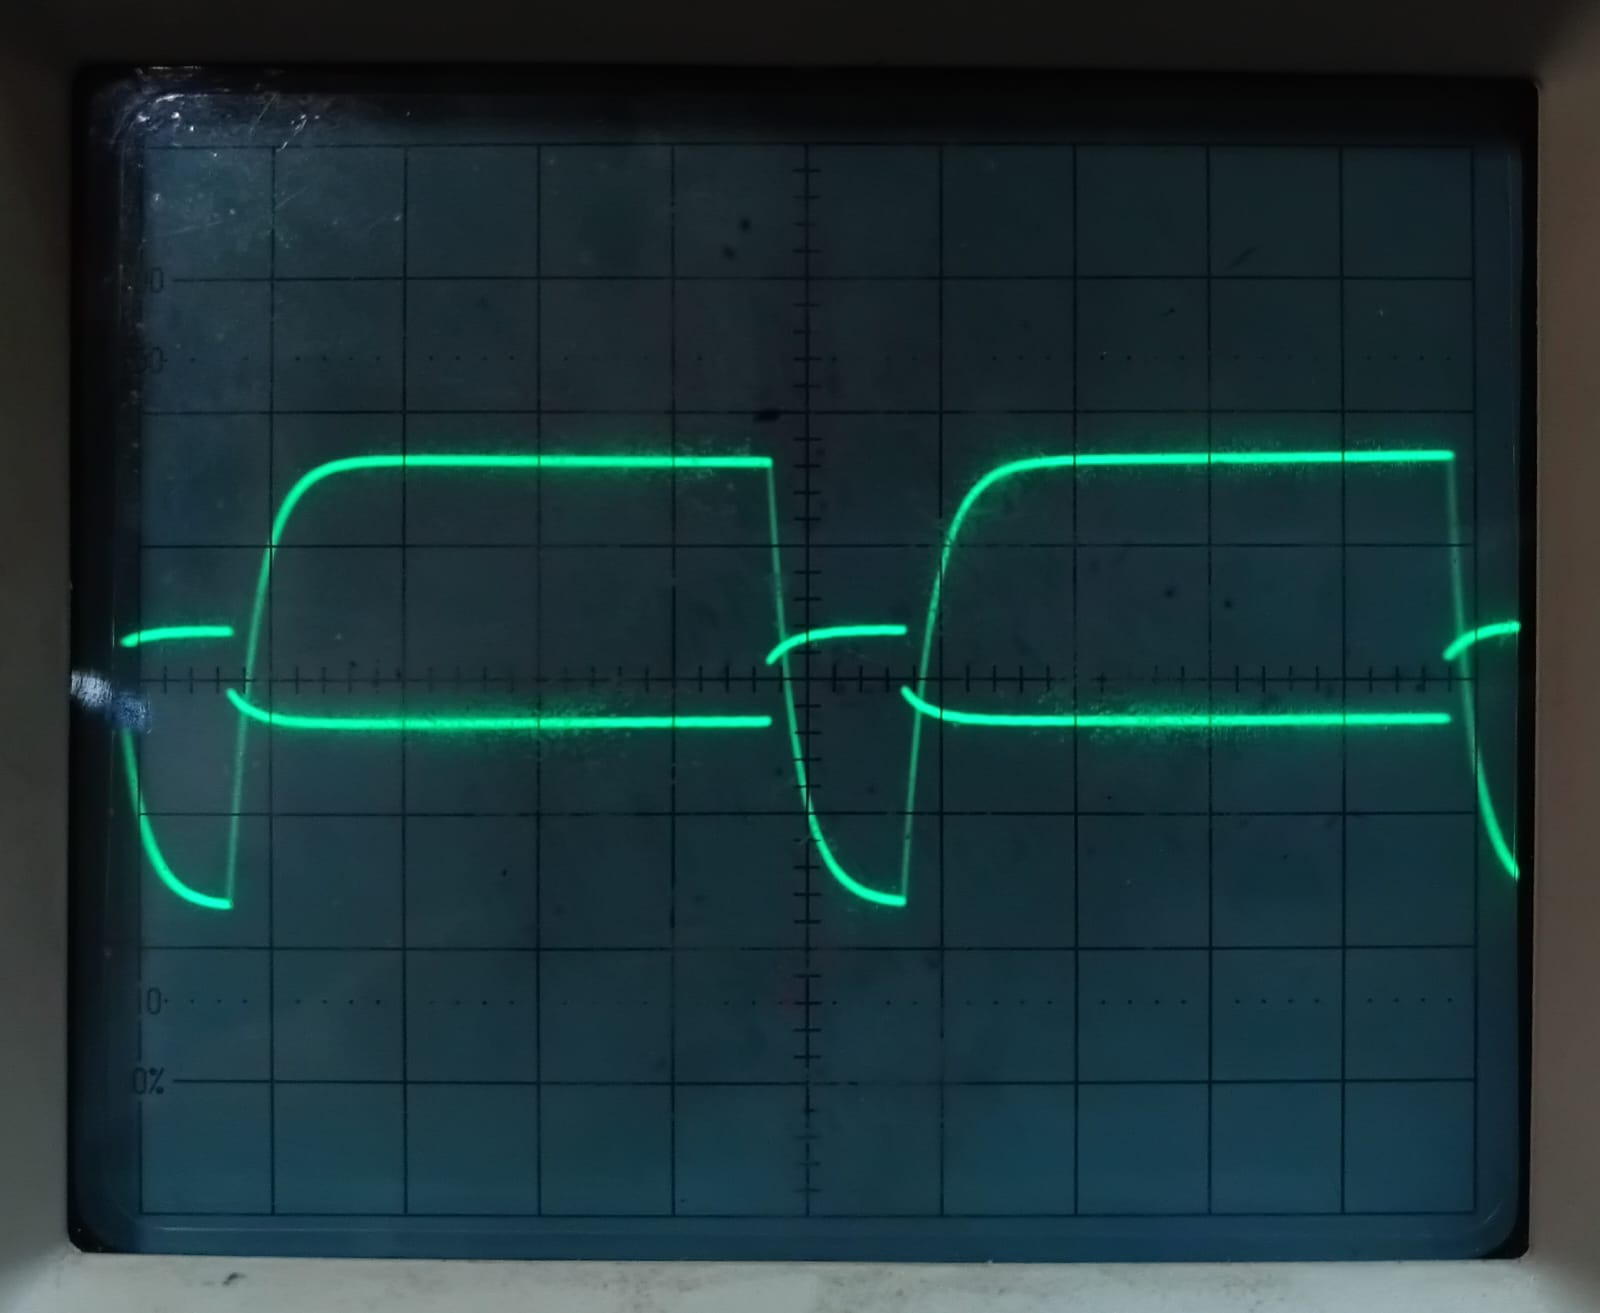
\includegraphics[width=0.8\textwidth]{Imagenes/dual10.jpeg}
        \caption{Modo Dual (DUAL)}
        \label{fig:dual10}
    \end{subfigure}
    \hfill
    \begin{subfigure}[b]{0.49\textwidth}
        \centering
            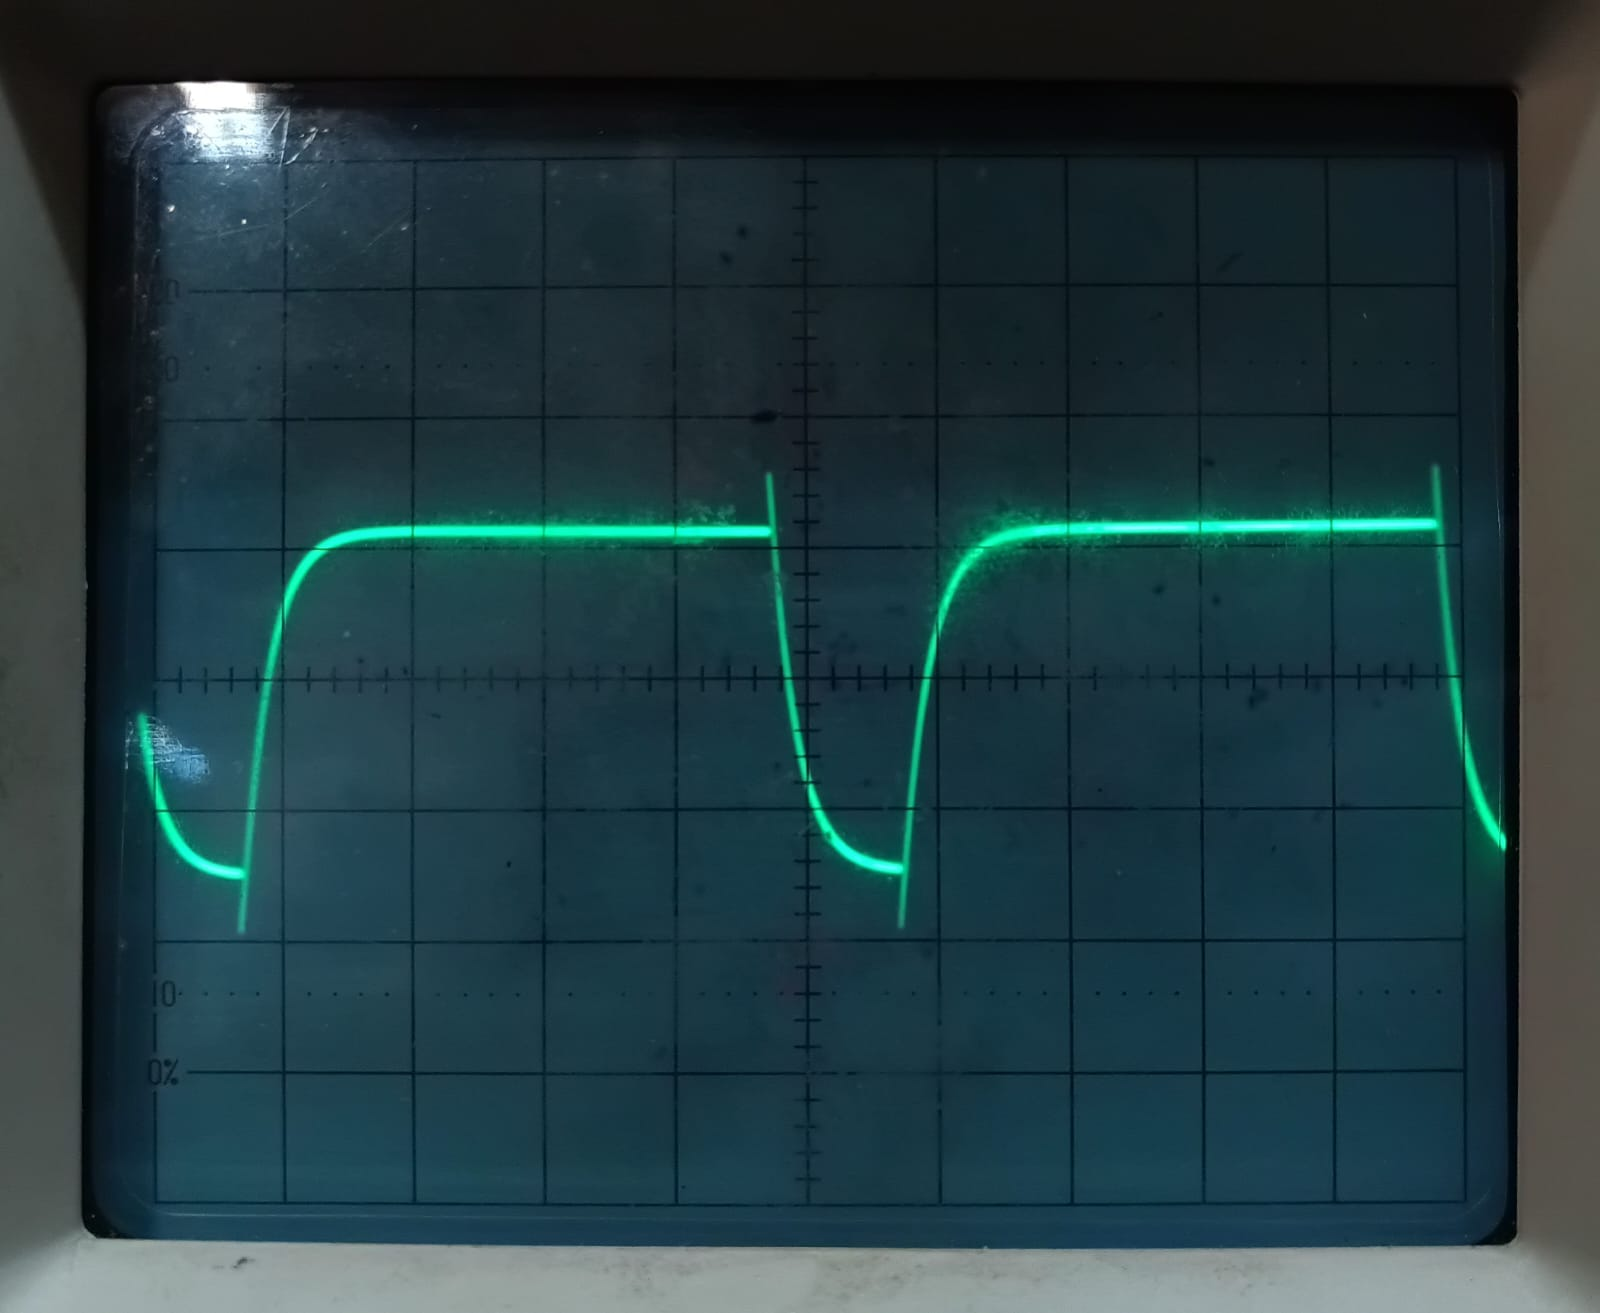
\includegraphics[width=0.8\textwidth]{Imagenes/suma10.jpeg}
        \caption{Modo Suma (ADD)}
        \label{fig:sum10}
    \end{subfigure}
    \caption{Señal en los distintos modos verticales}
    \label{fig:exp10}
    \end{center}
\end{figure}


Las características de esta señal son:

\begin{table}[H]
    \centering
    \scalebox{1}{
    \begin{tabular}{|c|c|c|c|c|c|}
    \hline
         Periodo (T) & Ancho (to) & Duty cycle & $V_{pp}$ & $V_{CC}$ & $V_{ef} = V_{pp} \cdot \sqrt{D - D^2}$ \\
    \hline
         1 ms & 0.8 ms & 80\% & 5.2v & 1V & 2.08V\\
    \hline
        \end{tabular}}
        \def\tablename{Tabla} 
        \caption{Características del tren de pulsos}
        \label{tab:trenPulsos}
\end{table}



